% Gravitational Camera: A Thought Experiment — working draft.
%
% This file is the single source for the paper. The website renders it with
% pandoc, so stay inside the subset the site understands: sections, \paragraph,
% paragraphs, equation/align with \label, figure, figure* (spanning both
% columns), table, quote (shown as a
% plain-language aside), itemize/enumerate, \cite, \ref, \eqref, \emph,
% \textbf, \footnote. No TikZ, no custom environments.
\documentclass[aps,prd,twocolumn,nofootinbib,floatfix]{revtex4-2}
\usepackage[T1]{fontenc}
\usepackage{lmodern,microtype}
\usepackage{amsmath,amssymb,graphicx}
\usepackage[hidelinks,pdfusetitle]{hyperref}
\usepackage{gcpaper}
% Shared notation. Plain \newcommand only, so pandoc can expand these for the web.
\newcommand{\tE}{\mathcal{E}}
\newcommand{\tB}{\mathcal{B}}
\newcommand{\TT}{\mathrm{TT}}
\newcommand{\dd}{\mathrm{d}}
\newcommand{\kB}{k_{\mathrm{B}}}
\newcommand{\SNR}{\mathrm{SNR}}


\begin{document}

\title{Gravitational Camera: A Thought Experiment}
\author{Mostafa ‘Neo’ Mohsenvand}
\noaffiliation
\date{Working draft, 16 November 2026}

\begin{abstract}
Suppose gravitational-wave detectors could be made arbitrarily small and
arbitrarily sensitive, and a camera were built with one at every pixel. What
would it see? A pixel records ten numbers, the electric and magnetic parts of the
tidal field, where a sensor of light records six and a wave of either kind
carries four. We show what the extra numbers buy. Written as one complex matrix,
a reading splits into four numbers that no observer can change, three that
orient the field and three that give the velocity of its rest frame. One pixel
therefore reads its own velocity through an unknown scene, at any speed; it
detects motion within the scene however it moves itself; it tells one body from
two and a wave from a pull; it gives a moving body's sideways velocity exactly,
at any speed; it separates two waves crossing it at one instant, three at one
frequency and four over time, where a sensor of light separates one, two and
two; it ranges a wave source out to a distance proportional to the
signal-to-noise ratio; and it sees moving bodies where they are now, not where
they were. One reading of any metric wave gives its speed and all six
polarizations a metric theory allows. An array forms an image in three regimes.
At everyday frequencies the camera sees the changing pull of nearby mass,
through any obstacle, but with a blur that shrinks only as the logarithm of its
sensitivity. In the waves radiated by moving bodies, a compact, slowly moving
body is an unresolved point. Only in the faint thermal radiation of matter are
sharp images possible, and there the world is transparent and self-luminous. No
broadband lens, mirror or shadow exists for such a camera, short of a black
hole, so its images are computed, not focused. Turned to the sky, the same
equations, solved in closed form, show the field of a pair of black holes
changing from Newton's pull to waves at a sixth of their wavelength, the memory
an explosion leaves, the Galaxy's centre outshining the rest of the millihertz
sky, and, if the early universe was hot enough, a primordial graviton glow at
$0.905\,\mathrm{K}$ in which black holes are the only shadows. This is a thought
experiment, not a proposal for an instrument. The draft is incomplete, and its
claims of novelty are provisional until the literature has been read in full.
\end{abstract}

\maketitle

\section{Introduction}\label{sec:introduction}

\begin{quote}
\textbf{In plain words.} Every camera we use records light. Light is stopped by
walls, by rock and by the body of the Sun. Gravity is not stopped by anything.
This paper asks what a camera would show if it recorded gravity instead of
light.

One instrument already records gravity in this way.
\textbf{\href{https://en.wikipedia.org/wiki/LIGO}{LIGO}} is an observatory with
two arms, each four kilometres long. It detects
\textbf{\href{https://en.wikipedia.org/wiki/Gravitational_wave}{gravitational
waves}}: ripples in space that moving masses send out, and that stretch and
squeeze everything they pass through. LIGO gives one number at each moment, so
in the language of photography it is a camera with a single pixel. This paper
imagines a camera in which every pixel is such a detector, made as small and as
sensitive as we like. It then asks what picture that camera would give of an
ordinary scene, such as a room, a street or the ground under our feet.

Physics that is already well tested answers this question. Gravity is weak
everywhere except close to black holes and neutron stars. Where gravity is
weak, Einstein's theory of gravity becomes much simpler, because the gravity of
separate masses simply adds up. This simpler form of the theory is called
\textbf{\href{https://en.wikipedia.org/wiki/Linearized_gravity}{linearized
gravity}}. The camera does not respond to colour or brightness. It responds
only to where mass and energy are, to how they move, and to the pressure and
tension inside matter, which in Einstein's theory also produce gravity.

The camera can see in three different ways.
\begin{itemize}
\item \textbf{By the pull of nearby masses.} Close to an object, the camera
feels the object's gravity directly. It therefore sees the mass itself, and
walls do not block the view. The picture is blurred, however, and a better
detector sharpens it only very slowly. For example, a detector a thousand times
more sensitive narrows the blur only from about $24^\circ$ to about $14^\circ$.
(A blur of $24^\circ$ is roughly the width of an outstretched hand held at
arm's length.)
\item \textbf{By the gravitational waves of moving objects.} A spinning or
orbiting object sends out waves that are far longer than the object itself. A
wave cannot show details smaller than its own wavelength, so the camera sees
such an object as a single point, with no shape.
\item \textbf{By the gravitational glow of warm matter.} Heat makes atoms
jiggle, and jiggling masses send out very weak gravitational waves. These waves
are as short as infrared light, so in principle they could give pictures as
sharp as those of an infrared camera. Matter hardly absorbs them, so solid
matter is transparent to them. At midnight, a camera pointed at the ground
would see the Sun's core shining through the Earth. The glow is extremely
faint, however. It arrives as
\textbf{\href{https://en.wikipedia.org/wiki/Graviton}{gravitons}}, the smallest
possible packets of gravitational-wave energy, just as light arrives as
photons. So few gravitons arrive that a whole lifetime of collecting would give
only a very coarse picture.
\end{itemize}

No lens or mirror can be made for gravitational waves, because matter barely
affects them. The camera must therefore compute its pictures from what its
pixels record. A single pixel also turns out to measure much more than one
would expect. For example, it can find its own velocity.

The last part of the paper asks how much the gravity outside a body reveals
about its inside. Newton's
\textbf{\href{https://en.wikipedia.org/wiki/Shell_theorem}{shell theorem}} says
that a hollow shell and a solid ball of the same mass pull in exactly the same
way on everything outside them. For black holes, the
\textbf{\href{https://en.wikipedia.org/wiki/No-hair_theorem}{no-hair theorem}}
says that the gravity outside shows only the mass, the spin and the electric
charge. The paper's main result is that the gravity of an ordinary body can
reveal far more than Newton's theorem suggests. A single snapshot of the body's
gravity shows only certain overall features of how its mass is arranged. A
second mass that flies past the body, however, sets the body's parts moving and
leaves some energy in them. The passing mass loses that energy from its own
motion, so it ends up slightly slower. How much slower depends on where the
body's mass lies. The losses along many different paths that miss the body give
the body's density everywhere inside. A black hole, tested in the same ways,
reveals only its mass, its spin and its temperature.

Most of the effects in this paper are far too small for any instrument we could
build. The paper is a thought experiment about what gravity carries in
principle.
\end{quote}

Gravitational waves were first detected in 2015 by LIGO \cite{LIGO2016}, an instrument four
kilometres long that reports a single number at each instant. In the language
of photography it is a camera with one pixel. This paper takes that language
seriously. We suppose that such detectors could be made as small and as
sensitive as we please, place one at every pixel of a sensor, and ask what
picture results when the sensor is pointed at an ordinary scene: a room, a
street, the ground beneath our feet.

The question has an answer because gravity is simple where it is weak. Every
form of matter and energy produces it, in proportion to its energy (and, for
fast motion and for light, its momentum and stress too), whatever it is made
of, and nothing shields it. The weakness that makes gravity so hard to detect makes a
gravitational camera easy to reason about: we need only the linear theory, and
the stress and motion of the matter in view.

Our results are these.
\begin{itemize}
\item A pixel measures the \emph{tidal field}, ten numbers at each point
(Section~\ref{sec:pixel}). One component of it, which is what an interferometer reads, cannot tell a
passing wave from the pull of a nearby object, and for everyday scenes the pull
dominates.
\item What the camera sees falls into three regimes, set by how far the source
is compared with the wavelength it would radiate (Section~\ref{sec:regimes}).
\item In the near field the camera sees mass itself, moving or still, through
any obstacle. Its blur is a fixed fraction of the distance, and improves only
with the logarithm of the sensitivity, for clocks and accelerometers as much as
for tidal pixels; but mass is never negative, and a scene of a few bodies is
measured far more sharply than it can be drawn. A body's steady pull hides its
interior; its thermal tremor, at a known temperature, reveals it, and a tide
applied from outside does the same at any temperature (Section~\ref{sec:near-field}).
\item In the waves radiated by moving bodies, a compact body moving slowly is
smaller than its own wavelength and appears as a point
(Section~\ref{sec:waves}).
\item In thermal radiation the camera can be as sharp as an infrared camera.
Matter is transparent, and glows in proportion to its internal friction and a
power of its temperature, up to a limit that a sum rule sets for every material
(Section~\ref{sec:thermal}).
\item Matter cannot act as a useful lens, a mirror or a screen for gravitational
waves, so the image must be computed from what the pixels record
(Section~\ref{sec:no-lens}).
\item One pixel measures far more than a sensor of light at a point, and a few
pixels more still (Section~\ref{sec:one-pixel}). A pixel's ten numbers are four
invariants, the orientation of the field and the velocity of its rest frame, so
it reads its own velocity through an unknown scene and detects motion within it
whatever its own. It tells whether its field could come from a single round
body or a single wave, reads a moving body's position, velocity and mass exactly at any
speed, separates up to four waves crossing it (a count that one theorem gives
for a field of any spin), ranges a wave source, sees moving
bodies where they are now rather than where they were, and reads the speed and
all six polarizations of a wave in one reading. Its magnetic part separates a
wave from the pull of nearby objects at a fixed cost in noise, and supplies the
one scale the electric part lacks, so a single pixel ranges a moving mass; a
few pixels side by side measure distance from how the field varies.
\item The expected number of gravitons that arrive sets what there is to be
seen: a first image, with its budget, and the reason why nothing made of
matter could catch it (Section~\ref{sec:first-image}).
Section~\ref{sec:affordances} lists what the camera can do that light cannot.
\item On the scale of the sky (Section~\ref{sec:vistas}): the field of two
black holes in orbit changes, at a sixth of their wavelength, from the pull of
two bodies to the waves of one; a spherical explosion sends out no waves,
and a lopsided one leaves space permanently stretched;
the Galaxy's centre, hidden from light by dust, is the brightest part of the
millihertz sky; and if the Big Bang was ever hot enough to make gravitons in
equilibrium, the whole sky glows at $0.905\,\mathrm{K}$, shares the large
spots of the microwave background, and has nothing dark on it but black
holes.
\item What the field outside a body determines of its interior is one
subject, gravitational hair (Sections~\ref{sec:hair} to~\ref{sec:holography}). The field at one time
gives the harmonic part of the body's mass and no more; the field at two times
gives all of it, through the same logarithm; and a black hole at rest yields seven
numbers to the first measurement and only its temperature to the second; its
response to a changing quadrupolar tide has the inertia of a shell of its own
mass just outside its horizon, and its responses to the first three tides
together that of no distribution of positive mass. The ambiguity is that of Newton's shell
theorem, and it holds only to first order in the mass of whatever feels the
field. The second measurement can be a tide applied from outside, followed by
a weighing, or a single mass that flies past the body: the energy it leaves
behind is taken from its own motion, and the amounts lost on the paths that
miss the body give all of the body's density. This is what remains in
classical physics of the holography argued for quantum gravity.
How much is reached depends on the tide. Tides of degree up to $m$ give $m$
radial moments of the density in every angular sector and no more, so that
there are bodies which no quadrupolar tide tells apart to leading order and an octupolar tide
does; two tides applied in either order give the flow within the body; and
an impulsive gravitational wave reads, at any speed, the energy that crosses
each point of its front.
\end{itemize}

Figure~\ref{fig:sun-at-midnight} shows where this leads. An observer stands on
the night side of the Earth and looks down. In light there is only dark ground.
In thermal gravitational radiation the planet is a set of glowing shells, and
beyond it, shining straight through, is the core of the Sun.

\begin{figure*}
\centering
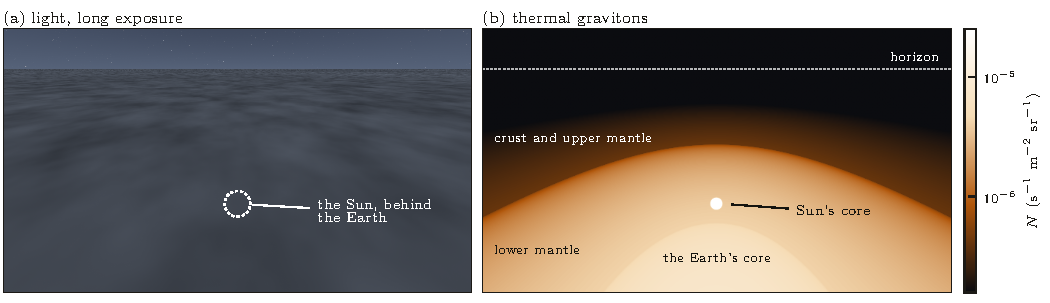
\includegraphics[width=\textwidth]{figures/sun-at-midnight.pdf}
\caption{The Sun at midnight, computed. An observer at latitude
$40^\circ$ north looks north and down, $33^\circ$ below the horizon, at local
midnight, with the same camera, $86^\circ$ from top to bottom, in both panels. (a) Ordinary light, exposed long enough to show the ground; the dotted
circle marks where the Sun lies, behind the planet. (b) Thermal gravitational
radiation: the expected number radiance $N(\hat n)$ of Eq.~\eqref{eq:column},
on a logarithmic scale. The ground is transparent. Lines of sight just below
the horizon cross only the crust and upper mantle and are faint; steeper ones
cross the hotter lower mantle, and those within $33^\circ$ of straight down,
at the foot of the picture, the core (Fig.~\ref{fig:earth-glow}). The Sun's core, $50^\circ$ below the horizon, is
smaller than a pixel; its flux, under one graviton per square metre per second,
is spread over a spot a few pixels across, far brighter than the top of the
scale. Section~\ref{sec:first-image} gives the model and its
assumptions.}\label{fig:sun-at-midnight}
\end{figure*}

\paragraph{What is already known.} The ingredients exist separately. Gravity
sensors already map buried structures by their pull \cite{Stray2022}; small
gravimeters are being made cheap enough to be set out as the pixels of an
imager \cite{Middlemiss2016,Prasad2021}, and a patent calls an array of them a
gravity camera \cite{JordanHowell2021}. The designers of LIGO worked out how strongly a walking
person disturbs it \cite{ThorneWinstein1999}, and seismologists have recorded
the gravitational signal of an earthquake arriving before the shaking
\cite{Vallee2017}. Gravity gradiometry has been proposed for imaging the contents
of cargo containers \cite{Kirkendall2007} and for locating objects under water
\cite{WuTian2010}. Networks of pulsars are analyzed as imaging telescopes for
gravitational waves from the distant universe \cite{BoylePen2012}, the
gravitational radiation of the Sun has been calculated
\cite{GarciaCelyRingwald2025,Steane2024}, and the tidal field has been
visualized around black holes and simple sources \cite{Nichols2011}. Much of
the algebra of a single reading is known in other forms: the frame in which the
electric and magnetic parts share their axes, the principal observer, has been
built from the curvature's invariants
\cite{CostaWyllemanNatario2021,WyllemanCostaNatario2021}; the
cross product of the two parts is the curvature's super-Poynting vector
\cite{MaartensBassett1998}; curvature can be measured operationally with test
bodies and clocks \cite{ObukhovPuetzfeld2019}; and the
polarization of a harmonic wave, as a detector of both parts would record it at
one place, has been drawn as four points on the sky \cite{Bruno2019}. What we
add is a single account of what an ideal observer of the tidal field would
record of ordinary surroundings, followed from the near field to the radiation
field and the thermal glow, with the limits of each regime stated.

\section{What a pixel measures}\label{sec:pixel}

\begin{quote}
\textbf{In plain words.} You cannot feel gravity while falling freely, and
neither can a detector. What can be felt is the \emph{difference} in gravity
between one place and the next: it stretches things along one direction and
squeezes them along another. That stretching is all a gravitational detector
ever measures.
\end{quote}

A freely falling observer feels no gravitational field at their own position.
What remains measurable is how the field differs between nearby points: the
tidal field. For an observer at rest, with proper time $t$ and coordinates
$x^0 = ct$, $x^i$, it is the symmetric tensor
\begin{equation}\label{eq:tidal}
\tE_{ij} = c^2 R_{0i0j},
\end{equation}
where $R$ is the Riemann curvature tensor, with signature $-{+}{+}{+}$ and
$R^\alpha{}_{\beta\gamma\delta} = \partial_\gamma\Gamma^\alpha_{\beta\delta} - \dots$. The
factor $c^2$ gives $\tE_{ij}$ the units $\mathrm{s^{-2}}$. Two free particles separated by a
small vector $\xi^i$ accelerate relative to one another by
\begin{equation}\label{eq:deviation}
\frac{\dd^2 \xi^i}{\dd t^2} = -\tE_{ij}\,\xi^j .
\end{equation}
Figure~\ref{fig:tidal} shows what this does to a ring of free particles, and
Fig.~\ref{fig:tidal-field} the field around masses and in a wave.

\begin{figure}
\centering
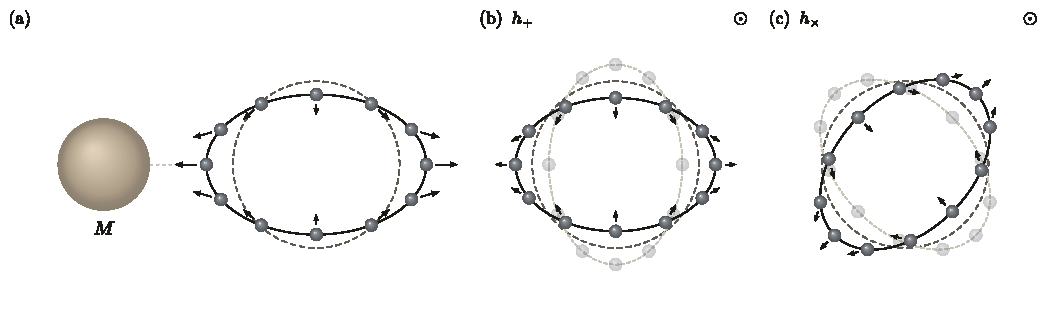
\includegraphics[width=\columnwidth]{figures/tidal.pdf}
\caption{What a pixel measures: a ring of twelve free test masses, distorted by the
tidal field, Eq.~\eqref{eq:deviation}, with each arrow the displacement of
its mass and the dashed circle the ring undisturbed; the distortions are
exaggerated. (a) Beside a mass $M$, the ring is stretched along the line to the
mass and squeezed across it, exactly twice as strongly along as across.
(b), (c) In a gravitational wave travelling toward the reader ($\odot$), of
polarization $h_+$ and $h_\times$: the ring is stretched and squeezed equally
along two perpendicular directions, which change places every half cycle (the
pale ring), and the two polarizations differ by a turn of $45^\circ$. The
planet's size and distance are schematic. A pixel records the size and
orientation of this distortion.}\label{fig:tidal}
\end{figure}

\begin{figure*}
\centering
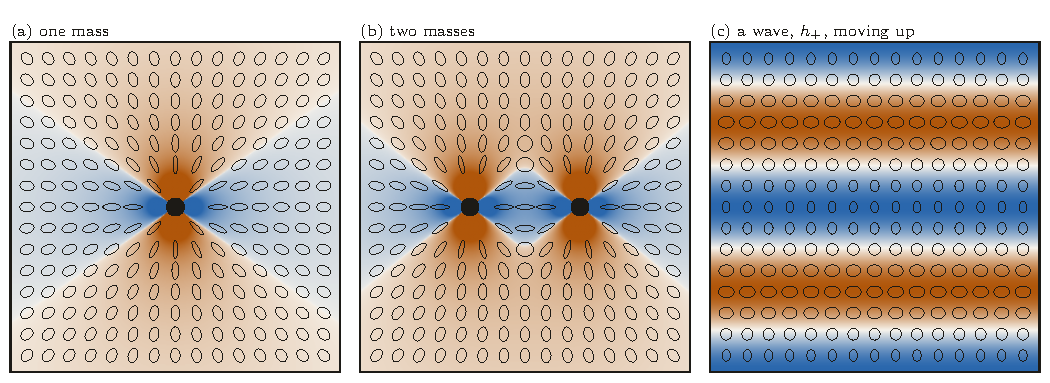
\includegraphics[width=\textwidth]{figures/tidal-field.pdf}
\caption{The tidal field itself. At points of a plane, a small ring of free
particles is drawn as the field distorts it (exaggerated, with the strength
compressed so that weak regions remain visible), over a map of one component:
$\tE_{zz}$ (up the page) in (a) and (b), $\tE_{xx}$ (across) in (c). Orange
marks a stretch along that axis (the component negative, by
Eq.~\eqref{eq:deviation}), blue a squeeze (positive). (a) One mass: every ring is
stretched toward it. (b) Two masses: midway between them the ring is stretched
along the line joining them and squeezed across it. (c) A plane wave of
polarization $h_+$ travelling up the page: bands of stretch and squeeze across
the direction of travel alternate every half wavelength, and nothing happens
along it. A pixel records one such ring, in three dimensions.}\label{fig:tidal-field}
\end{figure*}

Two limits of Eq.~\eqref{eq:tidal} matter here. Close to slowly moving matter,
the tidal field is the second derivative of the Newtonian potential $\Phi$:
\begin{equation}\label{eq:newton}
\tE_{ij} = \partial_i \partial_j \Phi .
\end{equation}
For a body of mass $M$ at distance $r$ its size is $2GM/r^3$ along the line to
the body. Far from its source, in a gravitational wave of strain
$h_{ij}^{\TT}$ (in the transverse traceless gauge),
\begin{equation}\label{eq:wave}
\tE_{ij} = -\tfrac{1}{2}\,\partial_t^2 h_{ij}^{\TT} .
\end{equation}
An interferometer such as LIGO reads one component of $\tE_{ij}$, integrated
twice in time, as the fractional change $h$ in the length of its arms.

Such a detector therefore responds to the ordinary pull of a passing lorry and
to a wave from a distant collision, and nothing in its one reading tells them
apart. The pull is not small. A person of $70\,\mathrm{kg}$ standing one metre
away produces $\tE \approx 9\times10^{-9}\,\mathrm{s^{-2}}$. If they sway by
five centimetres once a second, the field changes by $3\,\delta r/r$ of
itself, about $1.4\times10^{-9}\,\mathrm{s^{-2}}$, which a detector reads as a
strain $h = 2\,\delta\tE/\omega^2 \approx 7\times10^{-11}$, where
$\omega = 2\pi f$ is the angular frequency, here $2\pi\,\mathrm{s^{-1}}$. The
waves LIGO detects have strains near $10^{-21}$. This is why people and
vehicles must be kept away from its mirrors \cite{ThorneWinstein1999}. The
signal that the observatory removes as contamination is the one that a
near-field camera records.

An ideal pixel records all of $\tE_{ij}$, and also its magnetic counterpart
\begin{equation}\label{eq:magnetic}
\tB_{ij} = \tfrac{1}{2}\,c^2\,\epsilon_{ipq}\,R_{pqj0},
\end{equation}
with $\epsilon_{123} = +1$, which describes how the field twists the axes of
nearby gyroscopes relative to one another \cite{Nichols2011}. In vacuum both
are symmetric and trace-free, so
a pixel yields ten numbers at each instant; with this normalization the two are
equal in size in a plane wave, and $\tB_{ij}$ is $\tE_{ij}$ turned by
$45^\circ$ about the direction of travel. Inside matter the Ricci part of the
curvature adds local information that a pixel in vacuum does not see: the
trace $\mathrm{tr}\,\tE = c^2R_{00} = 4\pi G\rho$ in the Newtonian limit, and an
antisymmetric part of the magnetic tensor, $\tB_{[ij]} = -(4\pi
G/c)\,\epsilon_{ijk}\,\rho v_k$ for matter of density $\rho$ flowing at
velocity $\mathbf v$, which points along the flow. The pixel is also assumed
not to rotate: a frame turning at angular velocity $\Omega$ feels a
centrifugal pseudo-tide of order $\Omega^2$, and the Earth's own turning gives
$5\times10^{-9}\,\mathrm{s^{-2}}$, some thirty thousand times the tide of the
Moon, so gyroscopes must hold the frame still. We call an array of such pixels a
gravitational camera.

\paragraph{What the premise asks.} A pixel of this kind is an old idea. The
gravitational compass, a cluster of free masses read against one another, was
proposed to measure the curvature piece by piece
\cite{Pirani1956,Szekeres1965}; a sphere with several transducers reads the five
numbers of $\tE$ at one place \cite{Forward1971,WagonerPaik1977}; and a detector
that reads all of $\tE$ has been designed \cite{Paik2016}. In the near field
the premise asks little more than exists. Tides are measured in eotvos,
$1\,\mathrm{E} = 10^{-9}\,\mathrm{s^{-2}}$, and the person a metre away is nine
of them. An atom gradiometer carried over a buried tunnel reaches
$20\,\mathrm{E}$ in ten minutes \cite{Stray2022}; a superconducting one in the
laboratory, $0.02\,\mathrm{E}$ in a second \cite{MoodyPaikCanavan2002}, a
signal-to-noise ratio of five hundred on that person; and a satellite has
carried one as sensitive around the Earth \cite{RummelYiStummer2011}. Two free
masses of a gram, a centimetre apart and read for a second at the standard
quantum limit, would resolve $6\times10^{-14}\,\mathrm{s^{-2}}$, a hundred
thousand times less than the person's tide. The magnetic part asks more. It
can be read by gyroscopes \cite{Nichols2011}, by a gradiometer in motion
\cite{BraginskyCavesThorne1977,MashhoonPaikWill1989} or by light sent both ways
around a loop \cite{Frauendiener2020}, and in a wave it already enters the
response of an interferometer, at first order in the length of its arms over
the wavelength \cite{BaskaranGrishchuk2004}; but near slow matter it is smaller
than the electric part by $v/c$. The waves of moving bodies and the thermal
glow ask far more again, and the glow asks for something that no matter can
supply (Section~\ref{sec:first-image}).

\paragraph{The Earth's own tide.} On the ground the largest tide is the
planet's own, $2GM/R^3 = 3.1\times10^{-6}\,\mathrm{s^{-2}}$ along the vertical,
three hundred times that of the person a metre away. It is steady and known,
and it is subtracted, as the empty room is in Section~\ref{sec:near-field}: the
rooms of this paper are what remains, or rooms in free fall far from any
planet. The planet's turning is in the reading too. A pixel at rest on the
equator moves with the ground at $\Omega R = 465\,\mathrm{m\,s^{-1}}$, over a
planet that turns beneath it, and the two together
(Eq.~\eqref{eq:magnetic-point} and the spin dipole of
Section~\ref{sec:near-field}) give it a magnetic part
$(3GM\Omega/cR^2)(1 - I/MR^2) = 4.8\times10^{-12}\,\mathrm{s^{-2}}$, with $I$
the planet's moment of inertia: seventy thousand times the magnetic part of a
person walking past a metre away at $1.4\,\mathrm{m\,s^{-1}}$. This too is steady, and it is a measurement:
one pixel on the ground reads $I/MR^2$, the number that tells a planet with a
core from one without (Section~\ref{sec:near-field}).

The two parts are best written as one complex matrix, $\mathcal W = \tE +
i\tB$, and Section~\ref{sec:one-pixel} shows how much a single pixel can read
from it. The sections in between follow an array of pixels through the regimes
in which a camera forms images.

\section{What one pixel knows}\label{sec:one-pixel}

\begin{quote}
\textbf{In plain words.} A light sensor records six numbers at a point and a
gravitational pixel ten, although a wave of either kind is described by only
four. The extra numbers are not idle. From one reading of one pixel, with no
lens and no second pixel, the field tells which way a wave came from, how many
bodies are pulling, how fast the pixel itself is moving through the matter
around it, and where a moving body is now rather than where it was. Over time
it pulls apart several waves crossing it at once, and from how the field
departs from a perfect wave it tells how far away their source is. Light at a
point can do much less, for a reason that is a matter of algebra.
\end{quote}

A wave of light or of gravity reaching a point is described by four numbers: two
for its direction and two for the strengths of its two polarizations. A sensor
of light at a point records six, the electric and magnetic fields; a
gravitational pixel records ten, Eqs.~\eqref{eq:tidal} and~\eqref{eq:magnetic}.
This section shows what the six extra numbers buy. Most of it follows from
writing them as one object.

\paragraph{One complex matrix.} In vacuum $\tE$ and $\tB$ are real, symmetric and
trace-free. Together they form the complex symmetric trace-free matrix
\begin{equation}\label{eq:W}
\mathcal{W} = \tE + i\,\tB ,
\end{equation}
five complex numbers. Two facts make this the natural form.

First, observers transform $\mathcal{W}$ by rotations of three-dimensional space with
complex angles. A pixel turned by a rotation $R$ reads $R\,\mathcal{W} R^{T}$. A pixel moving
with rapidity $\eta$ along a unit vector $\hat u$ (speed $c\tanh\eta$) reads
$\Lambda\,\mathcal{W}\Lambda^{T}$ with $\Lambda = \exp(i\eta\,\hat u\cdot\mathbf{L})$, where
$(L_k)_{ij} = -\epsilon_{kij}$ generates rotations: a change of velocity is a
rotation by an imaginary angle. (The Lorentz group is isomorphic to the group of
complex rotations, $SO(3,\mathbb{C})$; for the curvature this is the content of
Petrov's and Penrose's classifications \cite{Petrov2000,Penrose1960}.) The
eigenvalues of $\mathcal{W}$, and with them
\begin{equation}\label{eq:invariants}
I = \mathrm{tr}\,\mathcal{W}^2, \qquad J = \mathrm{tr}\,\mathcal{W}^3,
\end{equation}
are therefore the same for every observer at that point, however turned and
however moving.

Second, a plane wave is a perfect square. For a wave travelling along $\hat k$,
let $\mathbf{e}_1, \mathbf{e}_2$ span the plane across it with
$\mathbf{e}_1\times\mathbf{e}_2 = \hat k$, and let
$\mathbf{m} = (\mathbf{e}_1 + i\mathbf{e}_2)/\sqrt2$, a complex vector with
$\mathbf{m}\cdot\mathbf{m} = 0$. Since $\tB_{ij} = \epsilon_{ipq}\hat k_p\tE_{qj}$ in
the wave, and $\hat k\times\mathbf{m} = -i\mathbf{m}$,
\begin{equation}\label{eq:square}
\mathcal{W} = 2(\tE_+ - i\tE_\times)\,\mathbf{m}\mathbf{m}^{T},
\end{equation}
where $\tE_+$ and $\tE_\times$ are the wave's two polarizations, so that a wave's
$\mathcal{W}$ has rank one. Conversely the direction of travel is read from $\mathbf{m}$
as $\hat k = \mathrm{Re}(i\,\mathbf{m}\times\mathbf{m}^*)/|\mathbf{m}|^2$, which for
one wave of any polarization is the gravitational counterpart of the Poynting
vector:
\begin{equation}\label{eq:one-wave}
\hat n_i = -\,\frac{\epsilon_{ijk}\,\tE_{jl}\,\tB_{kl}}{\tE_{ab}\,\tE_{ab}} ,
\end{equation}
with $\hat n = -\hat k$ pointing from the pixel back to the source. The same
construction for light gives $\mathbf{E} + ic\mathbf{B} = a\,\mathbf{m}$, a vector
rather than a square; the difference between the two, a square against a single
power, is the difference between spin two and spin one, and it is the source of
almost everything below. Matter neither reflects nor absorbs gravitational waves
(Section~\ref{sec:no-lens}), so none of what follows is spoiled by echoes, as
direction finding with radio or sound is indoors.

\paragraph{Four stars.} Every reading has four directions of its own. Writing a
complex null vector by its stereographic coordinate $z$ on the sky,
$\mathbf{m}(z) = (1 - z^2,\, i(1 + z^2),\, -2z)$, the quartic equation
\begin{equation}\label{eq:stars}
\mathbf{m}(z)^{T}\,\mathcal{W}\,\mathbf{m}(z) = 0
\end{equation}
has four roots, four points on the sphere of directions around the pixel: the
principal null directions of the field \cite{Penrose1960}, which we call its
stars. For one plane wave all four coincide on its direction of travel. For one
body at rest they fall in two pairs, on the line to the body and opposite it.
Where two or more bodies pull, they are four distinct points. The same
distinctions can be read without solving anything, from the invariants: a
repeated eigenvalue, the mark of a single body, makes
$1 - 6J^2/I^3$ vanish, and a single wave makes $I = J = 0$ (Petrov's types D and
N). One reading therefore tells whether the field could be that of one body,
whether it is a pure wave, or whether it needs more. In the reference
implementation the quantity $1 - 6J^2/I^3$ is below $10^{-8}$, rounding, for a
single moving body, and $0.02$ for two bodies at comparable distances.
Light at a point has two stars, not four: its $\mathbf{E} + ic\mathbf{B}$ has
only one complex invariant.

\paragraph{Ten numbers: four invariants, three angles, three velocities.} A
reading whose eigenvalues are distinct can be written
\begin{equation}\label{eq:polar}
\mathcal{W} = P\,\mathrm{diag}(w_1, w_2, w_3)\,P^{T}, \qquad
P = R_0\,e^{iK_0},
\end{equation}
with $P$ a complex rotation ($P^TP = 1$), split into a real rotation $R_0$ and an
imaginary one. The three complex eigenvalues, which sum to zero, are four
numbers no observer can change. The rotation $R_0$ gives three angles, the
orientation of the field's own axes. The imaginary part,
$e^{2iK_0} = P^{\dagger}P$, gives three more: the velocity of the one frame in
which $\tE$ and $\tB$ share their axes, the field's own rest frame. Ten numbers,
read as four, three and three.

The consequences are immediate. For a scene of masses at rest, $\tB = 0$ in the
scene's frame, so its eigenvalues are real; a pixel moving through it at any
speed still finds real eigenvalues, and finds in $P$ the velocity of the scene
relative to itself. The pixel is a speedometer: it reads its own velocity through
an unknown room, at any speed, with no map of the room. In the reference
implementation, for a pixel moving at $0.6\,c$ past four unknown masses, the
rapidity is recovered to $4\times10^{-8}$. To first order in the speed, in the
principal axes of $\tE$ with eigenvalues $\lambda_a$,
\begin{equation}\label{eq:speedometer}
\tB_{bc} = \frac{v_a}{c}\,(\lambda_c - \lambda_b) \quad ((a,b,c)\ \text{cyclic}),
\qquad \tB_{aa} = 0 ,
\end{equation}
so a pixel whose readings carry white noise $\sigma$ on each component reads
each component of its velocity to within
$c\,\sigma/\sqrt2\,|\lambda_b - \lambda_c|$. A pixel that reads the tide of a
room, $10^{-8}\,\mathrm{s^{-2}}$ near a person, to one part in $10^{8}$, reads its
own speed to about two metres per second.

The converse is an alarm. A pixel moving through a static scene, however fast,
always finds real eigenvalues. If they are complex, something in the scene
moves relative to the rest of it, or turns: the pixel's own motion can never
set it off. The phase of the eigenvalues measures turning. Outside a spinning
body of mass $M$ and angular momentum $J_s = Mca$, the eigenvalues are
proportional to $(r - ia\cos\vartheta)^{-3}$, as in Kerr's solution
\cite{Kerr1963}, so their phase, $3a\cos\vartheta/r$ for $a \ll r$, reads the
spin along the line of sight; for the Earth seen from above a pole it is
$1.5\times10^{-6}$.

Light cannot do this. Its field at a point has only two invariants,
$\mathbf{E}^2 - c^2\mathbf{B}^2$ and $\mathbf{E}\cdot\mathbf{B}$, and in the frame
where $\mathbf{E}$ is parallel to $\mathbf{B}$ a boost along their common axis
and a turn about it change nothing. A sensor of light is at best a
two-dimensional speedometer. A single body does the same to gravity's field
(type D): coming straight at the pixel, even at $0.3\,c$, it shows no $\tB$ at
all, and its radial speed is unreadable. Two bodies, or one that is not round,
remove the blind spot.

\paragraph{A moving body, exactly.} The four stars of a single body moving at any
speed are its two pairs, displaced by aberration toward its direction of motion.
Their midpoint, as a vector, is exactly its velocity across the line of sight:
\begin{equation}\label{eq:star-velocity}
\tfrac12\,(\hat p_+ + \hat p_-) = \frac{\mathbf{v}_\perp}{c} ,
\end{equation}
with $\hat p_\pm$ the directions of the two pairs and $\mathbf{v}_\perp$ the
velocity across the line from the body to the pixel. The reference
implementation finds the two sides equal to $2\times10^{-7}$ at $0.9\,c$. The
ratio $|\tB|/|\tE| = \sqrt3\,v_\perp/c$ of Section~\ref{sec:separation} is its
first-order form. A body coming straight on shows no sideways velocity and
cannot be ranged (Section~\ref{sec:separation}), but because its tide grows as
$r^{-3}$, the pixel reads when it will arrive,
\begin{equation}\label{eq:contact}
-\frac{r}{\dot r} = \frac{3\,\tE_\parallel}{\dot{\tE}_\parallel},
\qquad
\frac{\tE_\parallel\,\ddot{\tE}_\parallel}{\dot{\tE}_\parallel^2} = \frac43 - \frac{r\ddot r}{3\dot r^2},
\end{equation}
and from the second ratio whether it is coasting ($4/3$), braking or driven.

\paragraph{Separating waves at one point.} Several waves crossing a pixel at
once add their matrices, and the algebra of squares lets one pixel pull them
apart.

At one instant, two waves give $\mathcal{W} = c_1\mathbf{m}_1\mathbf{m}_1^{T} +
c_2\mathbf{m}_2\mathbf{m}_2^{T}$, of rank two, so $\det\mathcal{W} = 0$: two real
conditions that tell two crossing waves from the pull of a mass, whose
$\det\mathcal{W} = -2(GM/r^3)^3$. The vector $\mathbf{v}$ with $\mathcal{W}\mathbf{v} = 0$ is
$\mathbf{m}_1\times\mathbf{m}_2$; the null vectors orthogonal to it are the
roots of one quadratic, and they are $\mathbf{m}_1$ and $\mathbf{m}_2$, which give
both directions and then both amplitudes. This is Sylvester's theorem on sums of
two fourth powers \cite{Sylvester1851} in the language of the sky. Light cannot
do it at all: a single wave already uses four of its six numbers.

At one frequency, three waves can be separated. Writing the reading as
$\mathcal{W}(t) = \mathcal{W}_+e^{-i\omega t} + \mathcal{W}_-e^{i\omega t}$, both parts are sums
over the same three squares, $\mathcal{W}_\pm = \sum_a \alpha_a^\pm\,
\mathbf{m}_a\mathbf{m}_a^{T}$, and
\begin{equation}\label{eq:pencil}
\det(\mathcal{W}_+ - \lambda\,\mathcal{W}_-) = \det[\mathbf{m}_1,\mathbf{m}_2,\mathbf{m}_3]^2
\prod_{a=1}^{3}(\alpha^+_a - \lambda\,\alpha^-_a) .
\end{equation}
Its three roots give the ratios $\lambda_a = \alpha_a^+/\alpha_a^-$; at each, one
wave drops out, the null vector of what remains is the cross product of the other
two $\mathbf{m}$, and cross products of those give all three directions. For a
circular binary seen at inclination $\iota$, $|\lambda| = \tan^{\pm4}(\iota/2)$,
so the roots also give the three inclinations. Three binaries in one frequency
bin, which a single interferometer cannot tell apart, are three stars to one
pixel (to $10^{-9}$ in the reference implementation).

Over time, four. If the waves come from fixed directions but carry any
waveforms at all, the readings span a subspace of the five-dimensional space of
matrices; for four waves it is four-dimensional, and there is one matrix $A$ with
$\mathrm{tr}(A\mathcal{W}) = 0$ for every reading. Each wave's $\mathbf{m}$ then lies on
two conics,
\begin{equation}\label{eq:four-waves}
\mathbf{m}^{T}\!A\,\mathbf{m} = 0, \qquad \mathbf{m}\cdot\mathbf{m} = 0 ,
\end{equation}
and two conics meet in four points: the four directions. For light the same
argument gives two. In general a point sensor of a field of spin $s$ separates
$s$ plane waves at one instant, $s + 1$ at one frequency and $2s$ from a time
history; for light, $1$, $2$ and $2$, the known limit for electromagnetic vector
sensors \cite{NehoraiPaldi1994,HochwaldNehorai1996}; for gravity, $2$, $3$ and
$4$. In the reference implementation four waves with random waveforms are
located to $10^{-14}$, and to $10^{-4}$ radian with noise of $10^{-4}$ of the
signal on every component over three hundred readings.

Uncorrelated sources can be separated from second moments alone. In the
frequency domain the two helicities occupy separate halves of the ten numbers,
and the brightness and the circular polarization of the sources give two
five-by-five matrices built from the same five steering vectors; when the
sources' circular fractions differ, diagonalizing one in the frame that whitens
the other separates five sources in closed form, with their directions,
brightnesses and circular fractions (checked in the reference implementation).

\paragraph{What one pixel sees of the sky.} For a sky full of independent
sources overlapping in frequency, what a pixel can learn at each frequency is
its ten-by-ten spectral matrix, one hundred real numbers. Split by helicity, it
holds three blocks: the brightness $I$ and the circular polarization $V$ of the
sky in two five-by-five Hermitian blocks, and the linear polarization in a
complex symmetric one. The brightness enters through the kernel
\begin{equation}\label{eq:pixel-kernel}
\begin{gathered}
\sum_{A=+,\times} e^{A}_{ij}\, e^{A}_{kl}
= P_{ik}P_{jl} + P_{il}P_{jk} - P_{ij}P_{kl},\\
P_{ij} = \delta_{ij} - \hat n_i \hat n_j ,
\end{gathered}
\end{equation}
a polynomial of degree four in the components of $\hat n$, so the pixel sees the
spherical harmonics of $I$ of degree four and below, twenty-five numbers; it
sees as many of $V$, and eighteen of the linear polarization, which carries spin
weight four and enters only at degree four. That is
\begin{equation}\label{eq:sky-count}
25 + 25 + 18 = 68
\end{equation}
numbers of the sky, all independent; the other thirty-two of the hundred vanish
for any sky of gravitational waves and are checks against sensor noise or
anything else. The brightness and the circular polarization never mix at one
pixel: one lives in the real part of the spectral matrix, the other in its
imaginary part. (They mix in the cross-correlation of two separated detectors
\cite{AllenOttewill1997,SetoCooray2004}, through the phase between them.) The
same count for a point sensor of spin $s$ gives $2(2s+1)^2 + 2(4s+1)$: $28$ of
$36$ for light. For sound, a pressure and a velocity, it is $9$ of $16$. All
three counts are checked in the reference implementation.

One of the sixty-eight numbers is the handedness of the whole sky. An isotropic
sky of brightness $I$ and net circular polarization $V$ puts exactly
$(V/I)\langle\tE\cdot\tE^*\rangle$ into the imaginary part of
$\langle\tE\cdot\tB^*\rangle$, so one pixel measures
whether the sky is chiral, which a single planar interferometer cannot
\cite{SetoTaruya2007}.

The rest of the sky is invisible to second moments. The twelve corners of a
regular icosahedron form a spherical design of degree five: they average every
polynomial of degree five or less exactly as the whole sphere does
\cite{Delsarte1977}. Twelve equal, unpolarized, independent sources at those
corners therefore give a pixel exactly the second moments of a uniform sky,
while six at the corners of an octahedron, a design of degree three only, do
not; the reference implementation finds the first pair equal to one part in
$10^{15}$. Sources that are not Gaussian say more: the fourth moments of the
pixel are kernels of degree eight, which no icosahedron averages. Two pixels a
wavelength apart tell the two skies apart as well, because their
cross-correlation carries the phase $e^{i\omega\hat n\cdot\Delta\mathbf x/c}$,
which no finite design averages exactly.

\paragraph{How far away is a wave source?} A single plane wave has no distance.
The field of a real source at distance $r$ is not quite a plane wave: it carries
terms falling as $1/r^2$, $1/r^3$ and beyond, organized by how they turn about
the line of sight \cite{Sachs1962}, and a pixel sees them. At one instant the
departure of the oscillating part of $\mathcal{W}$ from rank one, the ratio of its
second singular value to its first, is
\begin{equation}\label{eq:ranging-instant}
\frac{s_2}{s_1} = \frac{C(\iota, \theta)}{(kr)^2} + O\bigl((kr)^{-3}\bigr),
\end{equation}
not $1/kr$: the first correction only tilts the apparent $\mathbf{m}$, which at one
instant cannot be told from a tilt of the source. For two masses turning in a
circle, seen at inclination $\iota$ and wave phase $\theta$,
\begin{equation}\label{eq:ranging-C}
\begin{gathered}
C = \frac{2\sin^2\!\iota\,\sqrt{A^2 + B^2}}{D}, \qquad
B = 2\cos\iota\,\sin\theta\cos\theta,\\
A = (1 - 3\cos^2\!\iota)\cos^2\!\theta - 4\cos^2\!\iota\,\sin^2\!\theta,\\
D = (1 + \cos^2\!\iota)^2\cos^2\!\theta + 4\cos^2\!\iota\,\sin^2\!\theta,
\end{gathered}
\end{equation}
which is $2$ for any phase seen edge on and vanishes at the angle
$\cos^2\iota = 1/3$. Over a cycle more can be done. The two frequency parts
$\mathcal{W}_\pm$ depart from rank one by $2\tan^{\pm2}(\iota/2)/(kr)^2$, so that
$kr = [2\sqrt{s_1(\mathcal{W}_+)s_1(\mathcal{W}_-)}/s_2(\mathcal{W}_+)]^{1/2}$ needs no knowledge of the
inclination. And the first-order tilt, invisible at one instant, differs between
the two helicities: the directions read from the two parts differ by
\begin{equation}\label{eq:helicity-split}
\Delta\theta_\pm = \frac{8\,|\cot\iota|}{kr} .
\end{equation}
A difference of directions measured at signal-to-noise ratio $\rho$ ranges the
source out to $kr$ of order $\rho$, where the rank departure reaches only $kr$
of order $\sqrt\rho$. A source seen at $\rho = 10^{3}$ can be ranged out to
several hundred reduced wavelengths: at $100\,\mathrm{Hz}$, a few hundred
thousand kilometres. The
reference implementation checks Eqs.~\eqref{eq:ranging-C}
and~\eqref{eq:helicity-split} against the exact field of a turning pair to
within a few per cent at $kr = 80$ and $0.5$ per cent at $kr = 200$.

\paragraph{The camera sees the present.} The field of a body moving uniformly is
its static field carried along, so it depends on where the body is now. The
stretch axis of $\tE$ points at the body's present position, at any speed (to
$10^{-7}$ radian at $0.3\,c$ in the reference implementation), while its light
shows its position a light-travel time ago, displaced by the aberration angle,
about $v_\perp/c$. Near two masses in orbit the changing part of the field is
Newton's field of their present positions to order $(kr)^2$, while their
retarded positions would be off by $kr$ itself: at $kr = 0.1$, a tenth of a per
cent against ten per cent. The first-order retardation cancels because mass and
momentum are conserved. The gravitational Sun is therefore $20.5''$ ahead of the
optical Sun along its yearly path across the sky. Laplace took the absence of
gravitational aberration to mean that gravity is far faster than light; it is
what general relativity predicts \cite{Carlip2000}. A camera that sees mass sees
it on its own slice of simultaneity. When a body changes its motion, the field
goes on pointing at where it would have been until the news, travelling at the
speed of light as a wave, arrives.

\paragraph{Beyond general relativity, in one reading.} Other theories of gravity
allow up to six polarizations, and waves that travel at other speeds
\cite{EardleyLeeLightman1973}. For any plane wave of the metric, of any
polarization and phase speed $v_p$, the second Bianchi identity gives, with no
field equations assumed,
\begin{equation}\label{eq:bianchi-wave}
\tB_{ij} = \frac{c}{v_p}\,\epsilon_{ipq}\hat k_p\,\tE_{qj} .
\end{equation}
So one reading of $\tE$ (now with a trace, six numbers) and $\tB$ (with an
antisymmetric part, eight) gives the direction ($\hat k$ is the null vector of
$\tB$ from the left), the phase speed, all six polarizations, and five checks that
they belong to one wave. In general relativity $v_p = c$ and only the two tensor
polarizations appear. A massive graviton and a massive scalar differ even in
sign: with $n = c/v_p$, the helicity-zero wave of a Fierz--Pauli graviton
\cite{FierzPauli1939} has longitudinal and breathing amplitudes in the ratio
$-2(1 - n^2)$, a scalar wave $+(1 - n^2)$. These are checked against curvature
computed from the metric in the reference implementation. Testing general
relativity this way at the level of present bounds would need extraordinary
signal-to-noise ratios; what is new is that it needs only one point.

\paragraph{How precisely.} With white noise $\sigma$ on each of the ten numbers
and $\rho = |\mathcal{W}|/\sigma$, one pixel places one wave to within $1/\rho$ radian in
each direction, against $\sqrt2/\rho$ for a sensor of light at the same
signal-to-noise ratio; it reads its own velocity as given after
Eq.~\eqref{eq:speedometer}; and it ranges a moving mass with the precision that
Section~\ref{sec:separation} gives.

\paragraph{Matter at the pixel.} Inside matter the pixel reads the density
locally, whatever the matter is: in full,
$\mathrm{tr}\,\tE = 4\pi G(\rho + 3p/c^2)$, less $2\Omega^2$ if the pixel's frame
turns at $\Omega$. The dark matter around the Sun, $0.4\,\mathrm{GeV\,cm^{-3}}$,
gives $6\times10^{-31}\,\mathrm{s^{-2}}$, by its mass alone and with no other
interaction. Between two plates a micrometre apart the Casimir energy is
negative and its pressure large, and the trace is negative,
$-8\times10^{-30}\,\mathrm{s^{-2}}$. The cosmological constant gives
$-\Lambda c^2 = -1\times10^{-35}\,\mathrm{s^{-2}}$. Where radiation streams
through, as neutrinos from a supernova do, the trace gives its energy flux and the
antisymmetric part of $\tB$ its direction (Section~\ref{sec:pixel}), so that
one reading inside the passing shell points back to the star, even when the
collapse is perfectly spherical and sends out no waves at all.

\begin{table}
\centering
\begin{tabular}{p{0.46\linewidth}p{0.12\linewidth}p{0.13\linewidth}p{0.14\linewidth}}
At one point & Sound & Light & Gravity \\ \hline
Numbers recorded & 4 & 6 & 10 \\
Numbers no observer can change & -- & 2 & 4 \\
Own velocity readable, components & -- & 2 & 3 \\
Waves separated at one instant & 1 & 1 & 2 \\
Waves separated at one frequency & -- & 2 & 3 \\
Waves separated over time & 2 & 2 & 4 \\
Sky numbers per frequency (of) & 9 (16) & 28 (36) & 68 (100) \\
Direction of one wave, standard deviation & -- & $\sqrt2/\rho$ & $1/\rho$ \\
\end{tabular}
\caption{What a sensor at one point can know, for sound (pressure and velocity),
light (electric and magnetic fields) and gravity (the ten numbers of a pixel).
Separation counts are for plane waves from distinct directions; over time the
waveforms are arbitrary. A dash marks an entry that does not
apply.}\label{tab:one-pixel}
\end{table}

\section{Three regimes}\label{sec:regimes}

\begin{quote}
\textbf{In plain words.} Close to a moving magnet, a compass needle follows it
at once; far away, all that is left is a radio wave, fading with distance. These
are the \href{https://en.wikipedia.org/wiki/Near_and_far_field}{near field and
the far field}, and gravity has the same two, divided at about a sixth of a
wavelength from the source (the wavelength over $2\pi$). A body that moves once
a second would radiate waves $300{,}000\,\mathrm{km}$ long, so its near zone
reaches $48{,}000\,\mathrm{km}$. Everyday life happens in the near field.

Matter radiates in two ways: bodies in bulk motion at the low frequencies at
which they move, and hot matter at the very high frequencies at which its
molecules jostle. The camera therefore has three regimes: the near field, where
it sees the changing pull of mass and the image blurs with distance; waves from
moving bodies, in which a compact source is a point; and the thermal glow, which
could be sharp but is so faint that almost no
\href{https://en.wikipedia.org/wiki/Graviton}{gravitons} arrive. Three facts
explain most of what follows. Gravity has
\href{https://en.wikipedia.org/wiki/Spin_(physics)}{spin} two, so its field at a
point is a pattern of stretch and squeeze, not an arrow like that of light;
matter moves slowly compared with light; and matter is too spread out, its ratio
$GM/Rc^2$ tiny, to bend or block gravity's waves short of a black hole.
\end{quote}

What reaches a pixel depends on how the distance $r$ to the source compares
with the wavelength $\lambda = c/f$ of the radiation it would emit at frequency
$f$. Inside the \emph{near zone},
\begin{equation}\label{eq:nearzone}
r \ll \frac{\lambda}{2\pi} = \frac{c}{2\pi f},
\end{equation}
the field is the Newtonian one of Eq.~\eqref{eq:newton}, following the source
almost instantaneously. Outside it the field is radiation, Eq.~\eqref{eq:wave},
falling off as $1/r$. At $1\,\mathrm{Hz}$ the near zone reaches to
$48{,}000\,\mathrm{km}$; at $1\,\mathrm{kHz}$, to $48\,\mathrm{km}$.
Figure~\ref{fig:regimes} places familiar sources on this map.

\begin{figure}
\centering
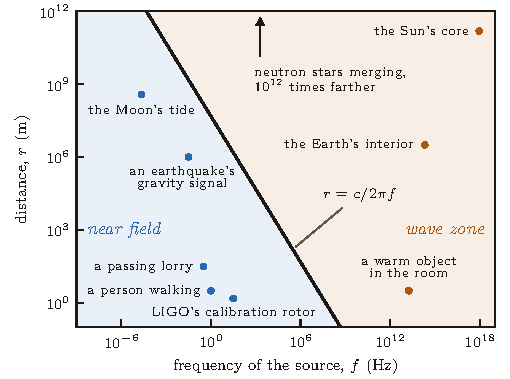
\includegraphics[width=\columnwidth]{figures/regimes.pdf}
\caption{Where sources lie. The diagonal is the edge of the near zone,
Eq.~\eqref{eq:nearzone}, $r = c/2\pi f$. Everything that moves mechanically,
from the tides to a calibration rotor beside a LIGO mirror, sits below it and
is seen through its changing Newtonian pull. Only radiation at thermal
frequencies, far to the right, reaches a nearby camera as waves short enough to
form sharp images; thermal sources are placed at the peak of their spectrum,
$f = 2.82\,k_BT/2\pi\hbar$.}\label{fig:regimes}
\end{figure}

Sources of radiation divide again. Bodies in bulk motion radiate at the
frequencies at which they move, which are low; hot matter radiates at the
frequencies of its molecular motion, which are very high. This gives the three
regimes of Table~\ref{tab:regimes}, taken in turn in the next three sections.

\paragraph{Spin, speed and compactness.} Almost everything the camera can and
cannot do follows from one property of gravity and two small numbers that
describe matter. \emph{Gravity has spin two}: curvature at a point is
a symmetric trace-free tensor, and in a wave it is the square
$\mathbf m\mathbf m^T$ of a complex null vector $\mathbf m$, where the field of
light is the vector itself. This gives the ten numbers of a pixel, the four
principal null directions of a reading, the separation of two, three and four
waves, the sixty-eight numbers of the sky that one pixel can measure and the
spin-two envelope of a sparse array (Section~\ref{sec:one-pixel}). \emph{Matter is slow},
$v/c \ll 1$: this puts the edge of the near zone, $\lambda/2\pi \sim L/(v/c)$,
far beyond any room, makes every compact moving body a point in its own
radiation (Section~\ref{sec:waves}), and makes the magnetic part of a near field
small, so that it is at once a clean channel for waves and a range-finder for
moving mass; only thermal motion reaches the frequencies at which the
wavelength is shorter than the body. \emph{Matter is tenuous}, its compactness
$GM/Rc^2 \ll 1$: this makes it transparent, so that hot matter glows
throughout (Section~\ref{sec:thermal}), and rules out lenses, mirrors,
absorbers and shadows short of a black hole (Section~\ref{sec:no-lens}), so
that images must be computed.

\begin{table}
\centering
\begin{tabular}{p{0.26\linewidth}p{0.4\linewidth}p{0.22\linewidth}}
Regime & What the pixel receives & What limits the image \\ \hline
Near field & the changing Newtonian pull of nearby mass & blur grows with distance \\
Waves from bulk motion & radiation from accelerating bodies & a compact source is an unresolved point \\
Thermal glow & radiation from molecular motion & almost no gravitons arrive \\
\end{tabular}
\caption{The three regimes of a gravitational camera.}\label{tab:regimes}
\end{table}

\section{The near field: mass seen through walls}\label{sec:near-field}

\begin{quote}
\textbf{In plain words.} The camera feels every nearby mass directly, through
anything in between, so it can see into a safe or weigh a lorry at a glance.
But the feeling blurs with distance, the way a hand under a thick blanket
shows only as a rough bump. Making the camera a million times more sensitive
makes the picture less than twice as sharp.
\end{quote}

In the near zone the camera measures the Newtonian tidal field of the scene as
it changes. Three properties follow at once. The field passes through all
matter, so no wall can screen a mass from the camera. Its strength is set by mass,
so the camera weighs what it sees. And it is present whether or not anything
moves, so a perfectly still scene is visible too.

\paragraph{How bright.} A body of mean density $\bar\rho$ and radius $R$ at
distance $r$ produces a tidal field of magnitude
\begin{equation}\label{eq:tidal-brightness}
\frac{2GM}{r^{3}} = \frac{8\pi G}{3}\,\bar\rho\,\theta^{3},
\qquad \theta = \frac{R}{r} .
\end{equation}
Tidal brightness is density times the cube of angular size. The Sun and the
Moon span the same angle in the sky, and the Moon, being denser, raises the
larger tide. A person one metre away spans a far larger angle than either,
and outweighs the Moon in the camera's view some fifty thousand times.

\paragraph{What the image is.} Summing Eq.~\eqref{eq:newton} over all the matter
in view, and grouping it by direction, gives the tidal field at the camera as
an integral over the sky,
\begin{equation}\label{eq:tidal-column}
\begin{gathered}
\tE_{ij} = G \int \dd\Omega\,\bigl(\delta_{ij} - 3\,\hat n_i \hat n_j\bigr)\,S(\hat n),\\
S(\hat n) = \int \rho(r\hat n)\,\frac{\dd r}{r} .
\end{gathered}
\end{equation}
The quantity $S$, which we call the \emph{tidal column}, is the mass along a
line of sight with each part weighted by the inverse of its distance;
Figure~\ref{fig:sky-integral} shows where the weighting comes from. The
integral starts a short distance $r_{\min}$ from the camera (a quarter of a
metre in the demonstrations), since matter at the camera itself would make $S$
diverge logarithmically, although not $\tE_{ij}$. A single pixel measures only
five numbers, the quadrupole of $S$ over the whole sky; an array, by comparing
the field from pixel to pixel, measures more.

\paragraph{What the image cannot show.} An array outside the matter it views
does not measure $S$ itself, because the field outside a body does not fix the
arrangement of mass inside it. A hollow shell and a solid ball of equal mass
produce the same field at every point outside both, however close. More
generally, adding to a body the density $\delta\rho = \nabla^2\chi/4\pi G$,
with $\chi$ any smooth function that vanishes outside it, changes the
potential by $\chi$ and so changes nothing outside \cite{YurtseverMarzbanMeila2011};
ordinary positive densities $\rho_0 \pm \epsilon\,\delta\rho$ make such pairs
out of real matter. The tidal column is therefore a rendering of a known
scene, the natural picture of what the camera responds to, and not a quantity
the camera could reconstruct uniquely. The near-field demonstrations show $S$
computed from the scene and blurred as described next. Other channels break
the ambiguity: the thermal glow shows a shell as a ring; a shell and a ball of
equal mass spinning at the same rate differ in $\tB_{ij}$ by the ratio of their
moments of inertia, $5/3$ (Section~\ref{sec:separation}), though at equal
angular momentum they are again alike; and a tide applied from outside probes
how the interior responds. The camera's position matters too: inside a closed
spherical shell it feels no tide from the shell at all, whatever its mass.

\begin{figure*}
\centering
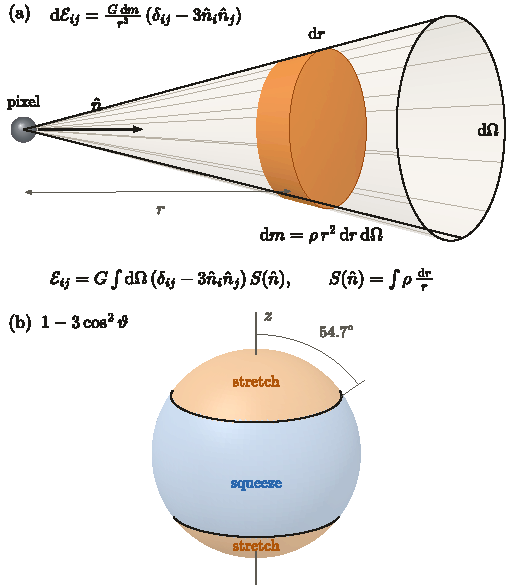
\includegraphics[width=\textwidth]{figures/sky-integral.pdf}
\caption{The sky integral, Eq.~\eqref{eq:tidal-column}. (a) A pixel at the apex
of a cone of directions $\dd\Omega$ about $\hat n$. The matter in the cone
between $r$ and $r + \dd r$, a piece of the cone bounded by two spherical caps
(orange), has mass $\dd m = \rho\,r^2\,\dd r\,\dd\Omega$ and adds
$G\,\dd m\,(\delta_{ij} - 3\hat n_i\hat n_j)/r^3$ to the tidal field. The $r^2$
of the volume cancels two of the three powers of $1/r$, so each line of sight
contributes its mass weighted by $\dd r/r$: the tidal column $S(\hat n)$. The
cone's width and $\dd r$ are exaggerated. (b) The sky around the pixel,
coloured by the sign of the weight $1 - 3\cos^2\vartheta$ with which one
component, $\tE_{zz}$, takes matter in each direction: matter in the orange caps,
within $54.7^\circ$ of the $z$ axis ($\cos^2\vartheta > 1/3$), stretches the
pixel along $z$; matter in the blue band squeezes it. The weight averages to
zero over the sky, which is why a uniform shell of matter around the camera is
invisible to it.}\label{fig:sky-integral}
\end{figure*}

\paragraph{What the image does show.} The ambiguity has an exact shape. For a
body whose outside is connected, every density splits in one way only into two
parts,
\begin{equation}\label{eq:split}
\rho = \rho_h + \frac{\nabla^2\chi}{4\pi G} ,
\end{equation}
where $\rho_h$ is harmonic inside the body, $\nabla^2\rho_h = 0$, and $\chi$
vanishes on the surface together with its gradient. The field outside fixes
$\rho_h$ completely and is blind to the rest \cite{Isakov1990}. The potential
outside is built from the moments $\int\rho\,h\,\dd V$ of the density against
functions $h$ harmonic in the body (the solid harmonics $r^\ell Y_{\ell m}$
about a point inside), and the second part has none of them, since
$\int h\,\nabla^2\chi\,\dd V = \int \chi\,\nabla^2 h\,\dd V = 0$. It follows that
any estimate of the interior that is linear in the data and treats every point
inside alike and independently, a white prior as in Eq.~\eqref{eq:wiener}, is
itself harmonic: it is built from the data's own kernels, which are. A harmonic
function has no maximum or minimum inside the region where it is harmonic. The
least assuming picture of an interior that a camera outside can draw, taking
the body's outline from light, therefore has its densest and its lightest
points on the surface. It can never show a core. Every round body appears as a
uniform ball of its mean density, and the layered Earth, seen from outside in
this way, as $5513\,\mathrm{kg\,m^{-3}}$ throughout.

Figure~\ref{fig:same-outside} shows three bodies with the same field outside. A
steel ball of radius $R$ holds a gold nugget of mass $m$ at the distance $s$
from its centre. The nugget's harmonic projection, the density harmonic in the
ball that has the same field outside, is
\begin{equation}\label{eq:harmonic-point}
\rho_h = \frac{m}{4\pi R^3}\sum_{\ell=0}^{\infty}(2\ell+1)(2\ell+3)\,
\Bigl(\frac{s r}{R^2}\Bigr)^{\ell} P_\ell(\cos\vartheta) ,
\end{equation}
with $\vartheta$ the angle from the nugget's direction; the sum has a closed
form, which the reference implementation uses. For $s = R/2$ it is a flush on
the wall nearest the nugget, $46\,m/4\pi R^3$ there, fifteen times the nugget's
mass spread evenly, fading toward the far wall, where it dips just below zero,
so that only the steel keeps it a real density. Poincar\'e's balayage sweeps the
same mass onto the surface as a skin of surface density
$m(R^2 - s^2)/4\pi R\,|\mathbf{x} - \mathbf{s}|^3$, thickest over the nugget. At
any sensitivity, a camera outside cannot tell the three apart.

\paragraph{What breaks the tie.} The three differ in one number that the
electric part cannot see, $\int\rho\,r^2\,\dd V$, the trace of the second
moment of the mass: $m s^2$, $\tfrac35\,m R^2$ and $m R^2$ for the nugget, the
flush and the skin ($r^2$ is not harmonic, so by Eq.~\eqref{eq:split} the
field outside carries no trace of it). The moment of inertia contains it,
$I_x = \tfrac23\int\rho\,r^2\,\dd V + \int\rho\,(r^2/3 - x^2)\,\dd V$, where the
second integral is harmonic and shared. Spun at the same rate about an axis
across the line to the nugget, the three therefore differ in angular momentum,
and so in the spin dipole of their magnetic fields
(Section~\ref{sec:separation}), by the gold's shares of the moment of inertia,
$0.25$, $0.48$ and $0.75\,mR^2$. The ball and the shell above, with
$\int\rho\,r^2\,\dd V = \tfrac35 MR^2$ and $MR^2$, are the simplest case. Spin
breaks only this one tie, since the moment of inertia is a single number. The
thermal glow, which sums along lines instead of reaching out as a potential,
would show the nugget as a spot, the flush as a gradient and the skin as a ring,
but the glow measures friction and temperature, not mass
(Section~\ref{sec:first-image}). A pixel inside the matter escapes the
ambiguity altogether, because there $\mathrm{tr}\,\tE = 4\pi G\rho$ reads the
density where the pixel is (Section~\ref{sec:pixel}).

Together the channels go further than any one. For the Earth the glow gives the
radius of the core, $3480\,\mathrm{km}$, from the kinks in its brightness
(Figure~\ref{fig:earth-inverted}); the electric part gives the mass; and the
magnetic part, with the rate of turning known, gives the moment of inertia,
$0.331\,MR^2$, the value the Preliminary Reference Earth Model is built to
match \cite{DziewonskiAnderson1981}. A two-layer Earth with that core, mass and
moment of inertia has a core of $12{,}500\,\mathrm{kg\,m^{-3}}$ and a mantle of
$4150\,\mathrm{kg\,m^{-3}}$. The reference model's core averages $10{,}900$; the
difference is the compression of the mantle under its own weight, which two
numbers cannot resolve.

\begin{figure}
\centering
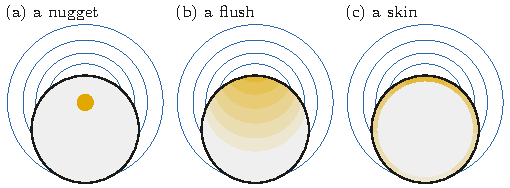
\includegraphics[width=\columnwidth]{figures/same-outside.pdf}
\caption{Same outside, different inside: three steel balls whose fields are
identical everywhere outside them. (a) A gold nugget halfway from the centre to
the wall. (b) Its harmonic projection, Eq.~\eqref{eq:harmonic-point}, the least
assuming interior that a camera outside could draw, shaded in bands that double
in density up to $46\,m/4\pi R^3$ at the near wall. (c) Its balayage: the
nugget's mass spread over the surface as a skin, drawn as a band of constant
width shaded in the same way, in steps that double in surface density up to
$6\,m/4\pi R^2$ over the nugget. Blue: equipotentials of the gold's share
of the field, drawn outside each ball (the steel's share is the same in all
three and is left out). They are the same in all three, and in (b) and (c) they
centre on a nugget that is not there. The reference implementation checks the
equality by integrating each body's potential directly.}\label{fig:same-outside}
\end{figure}

\paragraph{How sharp.} The space between scene and camera is empty, so the
potential there obeys Laplace's equation. Consider a pattern in the scene that
repeats across the line of sight with wavenumber $k$, at depth $z$ from the
sensor. Laplace's equation forces it to fade with height as
\begin{equation}\label{eq:evanescent}
\Phi \propto \cos(kx)\,e^{-kz} :
\end{equation}
fine detail dies away before it reaches the camera, and coarse detail
survives. To reconstruct the scene the camera must multiply each pattern by
$e^{kz}$, and its noise with it. If the largest features are recorded with
signal-to-noise ratio $\SNR$, patterns with $e^{kz} > \SNR$ are lost in the
noise, and detail finer than about $\pi z/\ln\SNR$ cannot be recovered.

The estimate can be made exact. Let a flat array at distance $z$ from a sheet
of sources with surface density $\sigma$ record the tidal field along its
normal with white noise of spectral density $N_0$. With $\Phi = -GM/r$ the
normal component above a mass is negative, a stretch, so we record
$d = -\tE_{zz}$. In Fourier space across the array the data are
\begin{equation}\label{eq:array-data}
\hat d(\mathbf k) = 2\pi G\,k\,e^{-kz}\,\hat\sigma(\mathbf k) + \hat n(\mathbf k),
\end{equation}
and the factor $k$ says that a uniform sheet is invisible: its pull is the
same at every pixel and at every height, so it has no tidal field at all.
Define the signal-to-noise ratio as the peak field of a
point mass $m$, $2Gm/z^3$, over the noise of the field averaged across a patch
of side $z$, $\sqrt{N_0}/z$: so $\SNR = 2Gm/(z^2\sqrt{N_0})$. Each Fourier
component of a point mass then stands above its own noise by
$s = \pi\,\SNR\;kz\,e^{-kz}$, and the best linear reconstruction (the Wiener
filter, which assumes the scene is a sheet of independent point masses) keeps
it with weight (taking as the prior a sheet of independent masses $m$, one
per area $z^2$, whose spectrum is $S_\sigma = m^2/z^2$)
\begin{equation}\label{eq:wiener}
H(k) = \frac{s^2}{1 + s^2}, \qquad s = \pi\,\SNR\;kz\,e^{-kz}.
\end{equation}
$H$ vanishes for a uniform scene, $k \to 0$, is close to one for patterns
between $kz \approx 1/\pi\SNR$ and $kz \approx 1$, and falls through one half
at $kz = q_c$, where
\begin{equation}\label{eq:cutoff}
q_c\,e^{-q_c} = \frac{1}{\pi\,\SNR},
\qquad
q_c \approx L + \ln L, \quad L = \ln(\pi\,\SNR)
\end{equation}
(10.1 against the exact 10.4 at $\SNR = 10^3$).
The image of a point is therefore close to the diffraction pattern of a round
pupil of radius $q_c/z$, $2J_1(x)/x$ with $x = q_c r/z$. The full width at half
maximum of this image, an amplitude and not its square, as an angle seen from
the array, is
\begin{equation}\label{eq:resolution}
\Delta\theta = \frac{4.43}{q_c}
\end{equation}
to within three per cent for every $\SNR \ge 100$ (for a single row of
sensors over a two-dimensional scene, $3.79/q_c$; the scene is then made of
line masses perpendicular to the row, and the potential obeys Laplace's
equation in two dimensions). Table~\ref{tab:resolution}
gives values, computed without approximation by the reference implementation
that accompanies the site, and Figure~\ref{fig:resolution-law} shows the law.

For an array at least as wide as the scene is deep, the angular blur does
not depend on distance or on the size of the array, only, through $q_c$, on the
logarithm of its sensitivity. A signal-to-noise ratio of a thousand gives
$24^\circ$; a million, $14^\circ$; $10^{30}$, still $3.4^\circ$. To match the
sharpness of the human eye, one arcminute, would take a signal-to-noise ratio
near $10^{6600}$. The first estimate $\pi/\ln\SNR$ is of the right size
everywhere, but it runs sharp at high sensitivity, because the image of a point
is wider than $\pi/q_c$. Figure~\ref{fig:nearfield} shows the reconstruction of
two masses, and the near-field demonstrations blur their images by
Eq.~\eqref{eq:resolution}. The same logarithmic limit is long familiar wherever
fields that obey Laplace's equation are continued back toward their sources: in
geophysics, where gravity and magnetic surveys are continued downward
\cite{Clarke1969,Parker1973}, and in near-field acoustic holography
\cite{MaynardWilliamsLee1985}.

\paragraph{A hand-held camera.} A camera much smaller than its distance from
the scene does worse. Inside a camera of width $D$, the part of the field that
varies over the sky with angular degree $\ell$ changes across the camera by a
factor $(D/2r)^{\ell-2}$ relative to the quadrupole, for a source at distance
$r$. Detail of degree $\ell$ therefore needs $\SNR \gtrsim (2r/D)^{\ell-2}$, and
\begin{equation}\label{eq:handheld}
\ell_{\max} \approx 2 + \frac{\ln\SNR}{\ln(2r/D)}, \qquad
\Delta\theta \approx \frac{\pi}{\ell_{\max}} .
\end{equation}
A camera ten centimetres across, looking at a lorry fifteen metres away with
$\SNR = 10^6$, sees detail of about $40^\circ$, not $14^\circ$. A single pixel,
$D \to 0$, sees the quadrupole alone. Widening the camera helps logarithmically
until it is about as wide as the scene is deep; beyond that,
Eq.~\eqref{eq:resolution} applies.

\paragraph{A blurred image is not a vague measurement.} The blur limits what
can be drawn of an arbitrary scene, not how precisely a simple one can be
measured. If the scene is known to hold a single point mass at depth $z$, an
infinite plane recording $\tE_{zz}$ with the noise above determines its
position to within $\sqrt{2/5}\,z/\mathcal{R}$ across and $z/\mathcal{R}$ in
depth, and its mass to within $\sqrt5/\mathcal{R}$ of itself, where
$\mathcal{R} = (\sqrt{3\pi}/4)\,\SNR$ is the signal-to-noise ratio of the whole
field pattern (the Cram\'er--Rao bounds with position and mass estimated
jointly, which we have checked by direct integration). At one metre and $\SNR = 10^3$ the mass is placed to within a
millimetre, while its image is $24^\circ$ wide. Two equal masses, by contrast,
can be told from one only when they are farther apart than about
$z/\sqrt{\mathcal{R}}$, because the difference they make grows as the square
of their separation. What limits the image is the variety of scenes allowed,
not the precision of the data.

\paragraph{How far can sensitivity go?} The premise of an arbitrarily sensitive
camera eventually meets the rest of physics. A heuristic argument, not a
theorem: a camera that fits within the distance $z$ to the scene, without
becoming a black hole, has a mass below $zc^2/2G$, so its energy of interaction
with a source of mass $M_s$ is below about $M_s c^2$. If quantum mechanics then
limits how quickly the camera's state can become distinguishable to a rate set
by that energy, as it does for a fixed coupling and a single measurement
task, over a time $\tau$ we would have $\SNR \lesssim M_s c^2\tau/\hbar$, with
$G$ and $z$ cancelling. For a person watched for the age of the universe this
is about $10^{70}$, a blur of $1.5^\circ$. On this estimate no near-field camera
could draw a face; making the estimate rigorous needs the coupling, the
resources and the discrimination task to be stated exactly.

\paragraph{How much a picture holds.} The resolution law says how fine the
detail of a near-field image can be. A different question, the one Shannon
asked of a telegraph line \cite{Shannon1948}, is how much the image can say:
how many bits the data carry about the scene. Equation~\eqref{eq:array-data}
answers it with no further assumption. Each Fourier component of the scene
reaches the array as a signal in additive Gaussian noise, standing above it by
the ratio $s$ of Eq.~\eqref{eq:wiener}, and components with different
$\mathbf k$ are independent. A real signal in Gaussian noise with power ratio
$s^2$ carries at most $\tfrac12\log_2(1+s^2)$ bits, a bound reached when the
signal is itself Gaussian, and a scene of area $A$ has $A\,\mathrm{d}^2k/(2\pi)^2$
real components in each $\mathrm{d}^2k$. Per area $z^2$ of the scene, with
$q = kz$, the data therefore hold
\begin{equation}\label{eq:capacity-integral}
C = \frac{1}{4\pi}\int_0^\infty q\,\log_2\!\left(1 + \pi^2\SNR^2 q^2 e^{-2q}\right)\mathrm{d}q
\end{equation}
bits about any scene with the spectrum of the prior of Eq.~\eqref{eq:wiener},
and a scene made of point masses carries somewhat less. Where $s > 1$, which
is for $q$ between about $1/\pi\SNR$ and $q_c$, the logarithm is close to
$2\log_2 s$; elsewhere it is small. Integrating $2q\log_2 s$ over that range,
with $\ln(\pi\SNR) = q_c - \ln q_c$ from Eq.~\eqref{eq:cutoff}, gives
\begin{equation}\label{eq:capacity}
C \approx \frac{q_c^3/3 - q_c^2/2}{4\pi\ln 2}
\end{equation}
to within three per cent for $\SNR \ge 10^3$ and half a per cent beyond
$10^{10}$.

The two terms have a plain reading. The patterns that survive the noise are
the components with $q < q_c$, and there are $q_c^2/4\pi$ of them per area
$z^2$; the rest of Eq.~\eqref{eq:capacity} is the number of bits each carries
on average, $(q_c/3 - \tfrac12)/\ln 2$, the mean of $2\log_2 s$ over them.
Greater sensitivity buys both more patterns and more bits in each, so with
$q_c \approx \ln\SNR$ the information grows, eventually, as
$(\ln\SNR)^3/12\pi\ln 2$: as the cube of the logarithm of the sensitivity. At
$\SNR = 10^3$ a near-field picture holds 38 bits per area $z^2$, about nine
patterns of four bits each. At $10^6$ it holds 200 bits; at $10^{30}$,
$1.6\times10^4$. At the heuristic ceiling of the previous paragraph, a person
watched for the age of the universe, it holds $1.8\times10^5$ bits, some 22
kilobytes, spread over 2{,}200 patterns of 80 bits each: about the size of a
thumbnail photograph, after sixty-seven orders of magnitude more sensitivity
(Figure~\ref{fig:capacity}). This is also why a blurred image and a precise
measurement are compatible. The data hold few bits, and a scene known to be
simple spends them all on a few numbers.

The camera's other channels scale differently, and the comparison shows what
is peculiar to the near field. A wave camera of width $D$ at wavelength
$\lambda$ resolves about $(D/\lambda)^2$ directions in each steradian, and each
carries about $\log_2\SNR$ bits: the aperture fixes the number of patterns, and
sensitivity adds bits only in proportion to its logarithm. In the near field
there is no aperture to fix the number of patterns; sensitivity sets it
through $e^{-kz}$, and that is why the power is three rather than one. A single
pixel, at the other extreme, is limited by geometry rather than noise: from a
sky of many overlapping sources it learns twenty-five numbers however
sensitive it is (Section~\ref{sec:no-lens}). And the thermal glow, recorded by
counting gravitons, is limited by their number: $N$ gravitons over $M$
resolution cells carry at most about $N\log_2 M$ bits. A camera a metre square
looking down at the Earth for a year counts about 1{,}750 of them in the model
of Section~\ref{sec:first-image}, so its picture of the planet's interior holds
a few kilobytes at any reasonable resolution.

\begin{table}
\centering
\begin{tabular}{rrrrrr}
$\SNR$ & $q_c$ & array & row & two points & $\pi/\ln\SNR$ \\ \hline
$10^{3}$ & 10.4 & 24.0° & 20.7° & 24.5° & 26.1° \\
$10^{6}$ & 17.8 & 14.1° & 12.1° & 14.6° & 13.0° \\
$10^{10}$ & 27.5 & 9.2° & 7.9° & 9.5° & 7.8° \\
$10^{20}$ & 51.1 & 5.0° & 4.2° & 5.1° & 3.9° \\
$10^{30}$ & 74.5 & 3.4° & 2.9° & 3.5° & 2.6° \\
$10^{60}$ & 144.3 & 1.8° & 1.5° & 1.8° & 1.3° \\
\end{tabular}
\caption{Blur of the near-field image. ``Array'': full width at half maximum
of the reconstructed image of a point, for a flat array, Eq.~\eqref{eq:resolution}.
``Row'': the same for a single row of sensors over a two-dimensional scene.
``Two points'': the smallest separation at which two equal point masses show
a dip between them in the array's image (Sparrow's criterion); because the
Wiener filter rolls off gradually, this slightly exceeds the full width, the
reverse of a sharp-edged pupil. The last column is the first estimate.}\label{tab:resolution}
\end{table}

\begin{figure*}
\centering
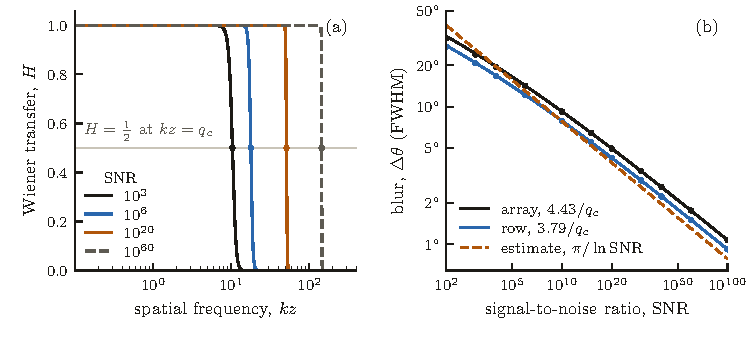
\includegraphics[width=\textwidth]{figures/resolution-law.pdf}
\caption{The exact near-field resolution law. (a) The Wiener filter $H$ of
Eq.~\eqref{eq:wiener} against spatial frequency, for four signal-to-noise
ratios: patterns coarser than $kz = q_c$ are kept almost whole, finer ones are
lost. Dots mark $H = \tfrac12$ at $q_c$, Eq.~\eqref{eq:cutoff}. Raising the
sensitivity from $10^{6}$ to $10^{60}$ moves the cutoff only from 18 to 144.
(b) The resulting blur, the full width at half maximum of the image of a
point, for a flat array ($4.43/q_c$) and a single row ($3.79/q_c$), with
values computed directly by the reference implementation (dots) and the first
estimate $\pi/\ln\SNR$ (dashed).}\label{fig:resolution-law}
\end{figure*}

\begin{figure}
\centering
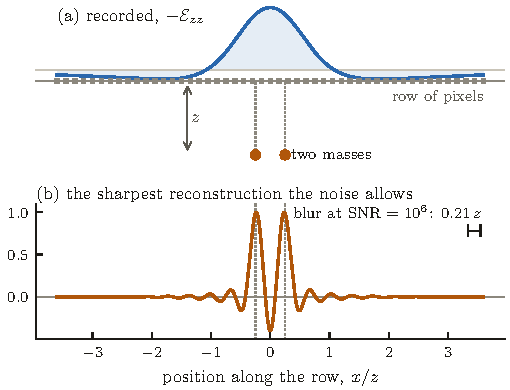
\includegraphics[width=\columnwidth]{figures/nearfield.pdf}
\caption{The near-field blur, for a row of pixels over a
two-dimensional scene: two line masses a distance $z/2$ apart at depth $z$, recorded
with signal-to-noise ratio $10^6$. (a) The geometry, to scale, and what the
pixels record: $\tE_{zz}$ along the row, a single smooth bump. (b) The best
reconstruction of the masses that the noise allows, the Wiener filter of
Eq.~\eqref{eq:wiener}, computed by the reference implementation; its ripples
are the price of discarding the detail that noise has swamped. The bar is the
blur, $0.21\,z$. On the website the sensitivity and the separation can be
changed.}\label{fig:nearfield}
\end{figure}

\begin{figure}
\centering
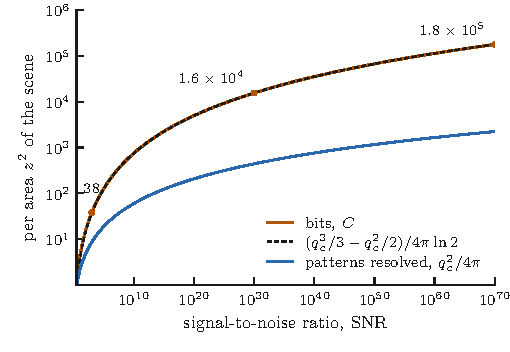
\includegraphics[width=\columnwidth]{figures/capacity.pdf}
\caption{How much a near-field picture holds, per area $z^2$ of the scene,
against the signal-to-noise ratio. Orange: the bits the data carry about the
scene, Eq.~\eqref{eq:capacity-integral}, computed by the reference
implementation. Dashed: the closed form of Eq.~\eqref{eq:capacity}, which lies
on it. Blue: the number of independent patterns resolved, $q_c^2/4\pi$. Raising
the sensitivity by sixty-seven orders of magnitude, from $10^3$ to $10^{70}$,
raises the information only from 38 bits to $1.8\times10^5$, about 22
kilobytes.}\label{fig:capacity}
\end{figure}

The logarithmic limit is the central result for the whole subject. The near field
is where everyday things are visible, and it can never be sharp. Sharp images
need waves.

\begin{figure*}
\centering
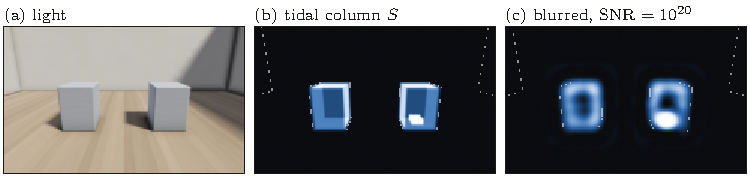
\includegraphics[width=\textwidth]{figures/locked-safe.pdf}
\caption{The locked safe, computed. Two identical steel safes
$3.5\,\mathrm{m}$ away; the right-hand one holds $320\,\mathrm{kg}$ of gold.
(a) Ordinary light, from the same camera. (b) The tidal column $S(\hat n)$ of
Eq.~\eqref{eq:tidal-column}, exact, with the empty room left out; white lines
mark the outlines that light shows. (c) The same, blurred by the point spread
of the Wiener reconstruction at a signal-to-noise ratio of $10^{20}$,
Eq.~\eqref{eq:resolution}: the gold still stands out through the steel.
Blurring $S$ in this way treats the scene as if it lay at a single depth; it
shows what an array as wide as the scene is deep could resolve, not a
reconstruction from simulated data (Section~\ref{sec:near-field}).}\label{fig:locked-safe}
\end{figure*}

\section{Waves from moving bodies}\label{sec:waves}

\begin{quote}
\textbf{In plain words.} Anything that is whirled, shaken or struck sends out
gravitational waves. But a wave cannot show detail smaller than its own
length, and these waves are longer than the thing that makes them by the same
factor that light is faster than the thing moves. A spinning flywheel is a
dot. The dot does carry a message: its polarization tells which way the wheel
is turning.
\end{quote}

Outside the near zone a source of mass quadrupole moment $Q_{ij}(t)$ produces
the strain
\begin{equation}\label{eq:quadrupole}
h_{ij}^{\TT}(t, r) = \frac{2G}{c^{4} r}\,
\ddot Q_{ij}^{\TT}\!\left(t - \frac{r}{c}\right),
\end{equation}
and radiates the power $P = (G/5c^{5})\,\langle \dddot Q_{ij}\,\dddot Q_{ij}
\rangle$. For two masses $m$ a distance $d$ apart, turning about their centre
at angular velocity $\Omega$,
\begin{equation}\label{eq:dumbbell}
P = \frac{8}{5}\,\frac{G m^{2} d^{4}\,\Omega^{6}}{c^{5}} .
\end{equation}
Two one-kilogram masses a metre apart, spun sixteen times a second, radiate
$4\times10^{-41}\,\mathrm{W}$: one graviton every fifteen years.

\paragraph{Every body is a point.} The waves of Eq.~\eqref{eq:dumbbell} have
twice the rotation frequency, so their wavelength is $\lambda = \pi c/\Omega$,
while the masses move at $v = \Omega d/2$. Hence
\begin{equation}\label{eq:unresolved}
\frac{\lambda}{d} = \frac{\pi}{2}\,\frac{c}{v} ,
\end{equation}
and the same holds, up to a factor of order one, for any body whose parts move
at speed $v$. The wavelength exceeds the body by the factor by which light
outruns it. No aperture can resolve an object smaller than the wavelength it
is seen by, so each moving body is a point in its own radiation.

\paragraph{What the point tells.} The radiation is not the same in all
directions, and it is polarized (Figure~\ref{fig:quadrupole}). Along the axis
of rotation it is strongest and circularly polarized, with the handedness of
the rotation; in the plane of rotation it is eight times weaker and linearly
polarized. From the polarization alone, a camera can read the axis and sense
of a rotor it cannot resolve.

\begin{figure}
\centering
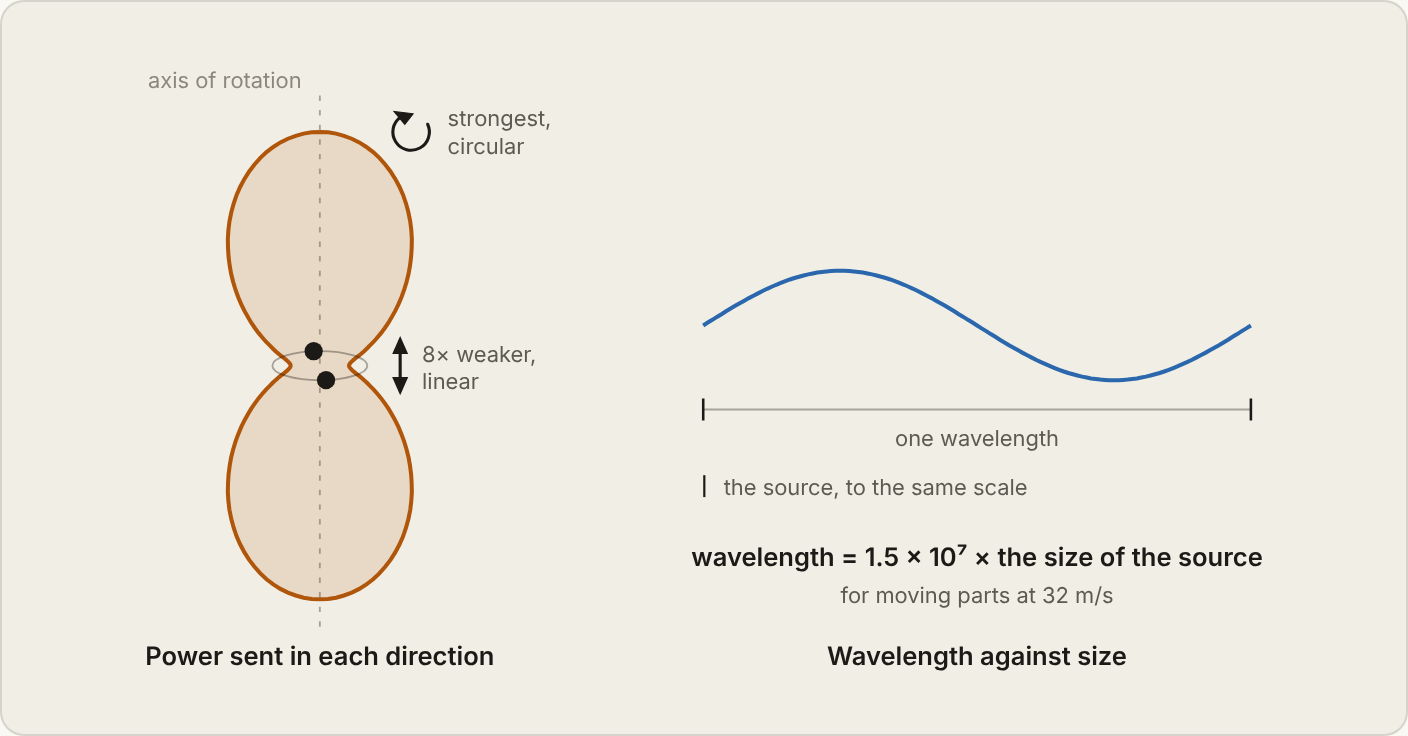
\includegraphics[width=\linewidth]{figures/quadrupole.png}
\caption{Radiation from a spinning pair of masses. Left: the power sent in
each direction, strongest along the axis of rotation. The small figures show
the polarization: circular along the axis, linear in the plane of rotation.
Right: the wavelength compared with the size of the source,
Eq.~\eqref{eq:unresolved}, for a chosen speed.}\label{fig:quadrupole}
\end{figure}

\paragraph{What does not radiate.} The source of the wave field is the part of
the stress that is transverse to the line of sight and has no trace. Steady
motion in a straight line has no changing quadrupole and radiates nothing. Nor
does anything that keeps spherical symmetry, however violently it pulsates.
And a pressure that is the same in all directions is pure trace: it is removed
exactly by the projection in Eq.~\eqref{eq:quadrupole}, a statement we have
verified numerically. The camera sees shear and lopsided motion, not pressure.

Because everyday speeds are so far below that of light, these effects cannot
be shown at human scale. The demonstrations that accompany this paper include
a clearly labelled mode in which the speed of light is lowered to walking
pace, so that the patterns of Figure~\ref{fig:quadrupole} become visible
around ordinary moving objects.

\section{The thermal glow: sharp, transparent, faint}\label{sec:thermal}

\begin{quote}
\textbf{In plain words.} Heat is molecules jostling, and jostling masses send
out gravitational waves of very short wavelength, short enough for sharp
pictures. Everything warm therefore glows, all the way through, and nothing
blocks the glow of whatever lies behind it. The picture is like an X-ray taken
by the object's own heat. It is also almost unimaginably faint.
\end{quote}

Sharp images need wavelengths shorter than the scene, and the only motion in
ordinary matter fast enough is thermal. At room temperature it radiates at
wavelengths of tens of micrometres, the same as thermal infrared light, so a
gravitational camera working there could be as sharp as an infrared one.

\paragraph{Absorption.} A gravitational wave crossing a medium shears it at
the rate $\tfrac{1}{2}\dot h_{ij}$. A medium of shear viscosity $\eta$ resists
with a stress $-\eta\,\dot h_{ij}$, which acts back on the wave as a source.
The wave equation becomes
\begin{equation}\label{eq:damped}
\ddot h_{ij} + \frac{16\pi G\,\eta}{c^{2}}\,\dot h_{ij} - c^{2}\nabla^{2} h_{ij} = 0 ,
\end{equation}
so the wave's energy decays at the rate $16\pi G\eta/c^{2}$, the result found
by Hawking \cite{Hawking1966}. Per unit length this is an absorption
coefficient
\begin{equation}\label{eq:alpha}
\alpha = \frac{16\pi G\,\eta}{c^{3}} .
\end{equation}
Here $\eta$ is the friction at the frequency of the wave; a viscosity measured
by stirring says little about a material's response at the $10^{13}$ cycles a
second of heat, as we discuss below. For water's everyday viscosity,
$\alpha \approx 10^{-37}\,\mathrm{m^{-1}}$: a wave would cross nearly
$10^{21}$ light-years of water before losing much of its energy.

\paragraph{Emission.} A medium that absorbs must also emit. With the Planck
radiance $B_\omega(T) = \hbar\omega^3/[4\pi^3c^2(e^{\hbar\omega/k_BT} - 1)]$,
summed over the two polarizations, Kirchhoff's law gives the power radiated per
unit volume, solid angle and frequency,
\begin{equation}\label{eq:kirchhoff}
j_\omega = \alpha(\omega)\, B_\omega(T) ,
\end{equation}
where $\alpha$ is the net absorption coefficient, absorption less stimulated
emission, and $j_\omega$ the spontaneous emission. We have checked
Eq.~\eqref{eq:kirchhoff} by a second route: computing the spontaneous
radiation directly from the thermal fluctuations of shear stress in a viscous
fluid, with the stress correlator taken in the unsymmetrized (Wightman) order
that the fluctuation--dissipation theorem relates to $\mathrm{Re}\,\eta$, gives
the same expression. For long wavelengths it is the known result
that a thermal plasma radiates gravitational waves in proportion to its shear
viscosity \cite{GhiglieriLaine2015}, and the same law has been applied to the
non-relativistic plasma inside the Sun, as one part of its gravitational
spectrum \cite{GarciaCelyRingwald2025}. What we add is its application to the
solids and liquids around us, whose friction at the frequencies of heat is
not that of a plasma.

Three consequences shape the image.
\begin{itemize}
\item \emph{Matter is transparent.} With $\alpha$ so small, nothing absorbs or
scatters. A pixel receives the sum of the glow of everything along its line of
sight (Figure~\ref{fig:line-integral}), and there are no shadows. Against a
background of radiance $I_{\mathrm{bg}}$, a body of optical depth $\tau$
changes what a pixel receives by $(B_\omega - I_{\mathrm{bg}})(1 -
e^{-\tau})$, which for ordinary matter is its own glow, $\tau B_\omega$, less a
negligible dimming of what lies behind.
\item \emph{Brightness is temperature times high-frequency friction.} What
sets a material's glow is how strongly it resists being sheared at the
frequencies of heat, which can be very different from its everyday viscosity
(see \emph{Gravitational colour}, below).
\item \emph{The glow is faint.} A person radiates of order $10^{-35}\,\mathrm{W}$
this way: at most one graviton in twenty million years.
\end{itemize}

\begin{figure}
\centering
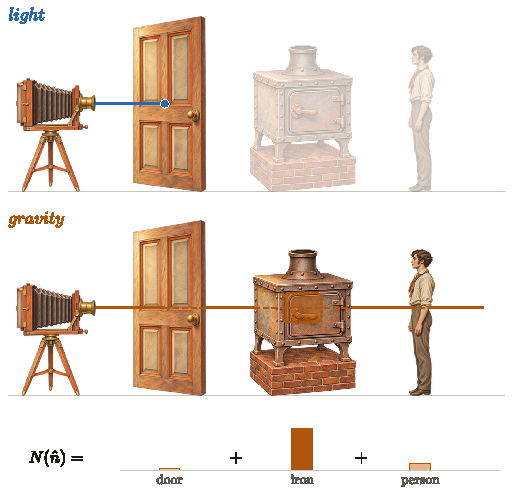
\includegraphics[width=\columnwidth]{figures/line-integral.pdf}
\caption{Two ways of forming a picture. A camera's line of sight passes
through a closed door, a closed iron furnace with a hot iron block inside, and
a person. In light it ends where it meets the door's face (the dot): a pixel
reports one point. Gravitational radiation passes through everything, so the
line runs on, dashed where a body hides it, and the hot block shows through the
furnace's walls. The pixel reports the sum along the whole line,
Eq.~\eqref{eq:column}: each body $k$ adds its number emissivity $j_{N,k}$ times
the length $\ell_k$ of the line inside it, shown below for illustrative
values in which the hot iron is far the brightest and the door, crossed only
through its thickness, adds little. The objects are illustrations, and their
sizes are chosen so that one level line crosses the middle of each.}\label{fig:line-integral}
\end{figure}

Figure~\ref{fig:closed-furnace} shows the first consequence at work. Two
closed steel furnaces hold the same block of iron, one at room temperature and
one at $1500\,\mathrm{K}$. They look the same and, to within the mass of their
heat ($\Delta U/c^2$, about $10^{-11}\,\mathrm{kg}$ per megajoule
\cite{Tolman1930}), weigh the same, so neither light nor the near field can
tell them apart at any ordinary sensitivity; the hot iron glows through the
steel. If the friction depended neither on frequency nor on temperature, the
number of gravitons emitted would grow as $T^3$ and the hot block would outshine
the cold one more than a hundredfold; the next paragraph explains why, for a
material whose stresses simply relax, this is an upper estimate.

\begin{figure*}
\centering
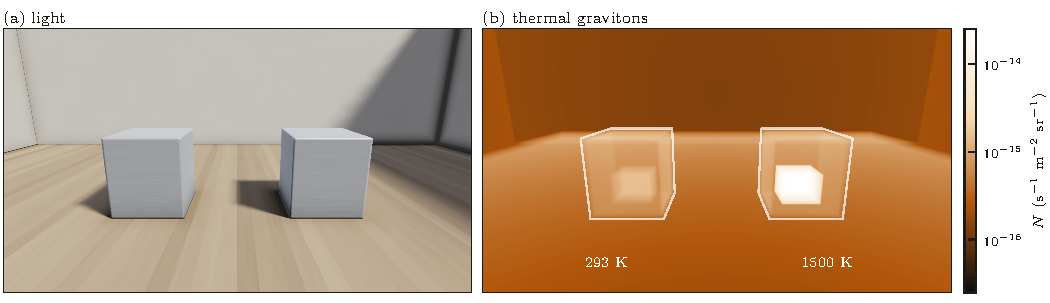
\includegraphics[width=\textwidth]{figures/closed-furnace.pdf}
\caption{The closed furnace, computed. Two closed steel furnaces
hold the same block of iron, one at $293\,\mathrm{K}$ and one at
$1500\,\mathrm{K}$. (a) Ordinary light: the two are identical. (b) The expected
thermal number radiance, Eq.~\eqref{eq:column}, from the same camera, on a
logarithmic scale, with the outlines that light shows. The hot iron glows
through its steel; the cold block cannot be told from its surroundings. The
room itself glows faintly, brightest where a line of sight crosses the floor
at a slant. The values assume the placeholder friction discussed in the
text.}\label{fig:closed-furnace}
\end{figure*}

\paragraph{Gravitational colour.} Equation~\eqref{eq:alpha} holds when the wave
is slower than the processes that produce viscosity. At the frequencies of heat
that is rarely so, and $\eta$ must be replaced by the dissipative part of the
material's shear response at the frequency of the wave, the real part of its
dynamic viscosity, $\mathrm{Re}\,\eta(\omega)$ \cite{BaymPatilPethick2017}. A
simple model shows how much this matters. A liquid whose stresses relax in a
time $\tau$ (Maxwell's model) has
\begin{equation}\label{eq:maxwell}
\mathrm{Re}\,\eta(\omega) = \frac{\eta_0}{1 + \omega^2\tau^2} ,
\end{equation}
so its everyday viscosity $\eta_0$ survives only below $\omega \approx 1/\tau$.
Above it the friction falls as $\eta_0/(\omega\tau)^2 = G_\infty^2/\eta_0\omega^2$,
where $G_\infty = \eta_0/\tau$ is the liquid's stiffness against sudden shear:
at a given stiffness, the more viscous liquid glows the less. Honey is viscous
because its molecules rearrange slowly; at the frequencies of heat that
rearrangement is frozen, and honey need not outshine water at all. In dense
matter the friction at those frequencies comes from much faster processes, and
an order-of-magnitude guess is $10^{-4}$ to $10^{-3}\,\mathrm{Pa\,s}$, which is
why we use $10^{-3}\,\mathrm{Pa\,s}$ as a placeholder. A crystal has no sound
waves above its Debye frequency, so above its Debye temperature its glow grows
more slowly than $T^3$ as well. Maxwell's model falls steadily with
frequency; a real material can have resonances in its losses, and then needs
its own spectrum of stress fluctuations, which may exceed this estimate in a
band. The spectrum of the glow therefore records a
material's mechanical losses, a kind of gravitational colour, and with a
frequency-dependent friction the number emissivity must be computed as
$j_N = \int \alpha(\omega)\,B_\omega\,\dd\omega/\hbar\omega$ rather than by
dividing the power by $2.70\,k_BT$.

Two consequences follow. The honey-and-water demonstration shows the contrast
that everyday viscosity would give, and is labelled as such. And temperature
cannot be read from the glow alone: a different temperature with a different
friction spectrum gives the same $j_\omega$, so a thermal gravitational image
measures temperature only when the material's response is known from elsewhere.

\paragraph{A glowing volume or a glowing outline?} Thermal radiation from the
vibrations of a solid has been calculated before
\cite{SchaeferDehnen1981,SchaeferDehnen1981erratum,DehnenRomeroSchaefer1984};
for an elastic sphere without internal damping its strength was found to grow
with the sphere's surface, not its volume. Which channel wins should depend on
how far a sound wave travels before it is damped: where that distance is much
shorter than the body, as in most solids at room temperature, the volume
emission of Eq.~\eqref{eq:kirchhoff} should dominate, while a cold, pure crystal
might glow at its surface. Both can be computed. In an elastic body without
loss a wave is absorbed only where the stiffness changes, at the surface, where
it launches sound \cite{Dyson1969}; for a sphere below its Debye temperature
the thermal glow that follows is \cite{DehnenRomeroSchaefer1984}
\begin{equation}\label{eq:surface-glow}
L_S = 4\pi R^2\,\frac{\pi^2}{24}\Bigl(1 + \frac{3c_T}{2c_L}\Bigr)
\frac{G\rho\,c_T^3\,(k_BT)^2}{\hbar c^5} ,
\end{equation}
with $c_T$ and $c_L$ the speeds of shear and compressional sound: by
Kirchhoff's law, a surface that absorbs the fraction
$\pi^2(1 + 3c_T/2c_L)\,G\rho c_T^3/c^3\omega^2$ of a wave, Dyson's absorption
with its constant. Friction inside, $\mathrm{Re}\,\eta = \rho c_T^2/\omega Q$ for
sound of quality factor $Q$, makes the volume glow by Eq.~\eqref{eq:kirchhoff},
with $L_V = V\,32\zeta(3)\,G\rho c_T^2 (k_BT)^3/\pi c^5 Q\hbar^2$, and
\begin{equation}\label{eq:volume-surface}
\frac{L_V}{L_S} = \frac{256\,\zeta(3)}{\pi^3\,(1 + 3c_T/2c_L)}\,
\frac{R}{\ell_s} ,
\end{equation}
where $\ell_s = Q\hbar c_T/k_BT$ is the distance a thermal phonon travels
before it is damped; the prefactor is $5.5$ for steel. Thermal phonons in
solids at room temperature travel nanometres, so ordinary bodies glow through
their volume: a steel ball of radius $10\,\mathrm{cm}$ at room temperature
glows $10^{-46}\,\mathrm{W}$ from its surface and, with $Q\approx10$ for its
thermal phonons, $7\times10^{8}$ times more from its volume. A pure crystal cooled until
its phonons cross it glows at its surface, in proportion to $T^2$ rather than
$T^3$, as Dehnen, Romero and Schäfer found. The reference implementation
checks both expressions by integrating Kirchhoff's law over the spectrum.

\section{A camera without a lens}\label{sec:no-lens}

\begin{quote}
\textbf{In plain words.} A glass lens works because glass slows light. Nothing
slows, bends or blocks gravitational waves enough to matter, so this camera
can have no lens, no mirror and no shutter. It does not need them. Each pixel
records the wave itself, crest by crest, and a computer can then combine the
pixels to do what a lens would have done.
\end{quote}

\paragraph{Nothing to build optics from.} Matter of density $\rho$ changes the
speed of a gravitational wave of angular frequency $\omega$ by the fraction
\cite{Peters1974}
\begin{equation}\label{eq:index}
n - 1 = \frac{2\pi G \rho}{\omega^{2}} ,
\end{equation}
which for steel at $1\,\mathrm{kHz}$ is $10^{-13}$, and falls as the square of
the frequency. A steel lens a metre thick would bring such a wave to a focus
only some $10^{13}$ metres away, beyond the orbit of Pluto; and since the wave
is three hundred kilometres long, a lens able to act on it at all would have
to be far larger. The same number sets reflection: by our estimate a steel
wall, however thick, returns less than $10^{-27}$ of the energy of a kilohertz
wave. Absorption is weaker still
(Section~\ref{sec:thermal}).

A mass does bend passing waves by its gravity, exactly as it bends light, by
the angle $4GM/bc^{2}$ for a ray passing at distance $b$. Used as a lens, the
Earth has a focal length of fifteen thousand times the distance to the Sun,
and a focal ratio near $10^{8}$. In each case the strength of the effect is
set by the same number, the compactness $GM/Rc^{2}$ of the body, which is
$7\times10^{-10}$ for the Earth and of order one only for a black hole. Bounds
of this kind on absorption are known \cite{Loeb2020}. We expect a single
statement to cover all four effects: no body much less compact than a black
hole can focus, reflect, absorb or block gravitational waves appreciably.
Proving it is part of this work. In the gravitational sky, only black holes
cast shadows.

\paragraph{The computed image.} The camera does not need optics, because its
pixels record more than a light sensor does. A light sensor registers only
the energy that arrives. A gravitational pixel registers the field itself,
with its phase. Waves from a direction $\hat n$ reach different pixels at
different times, and the image is made by undoing those delays and adding:
\begin{equation}\label{eq:beam}
I(\hat n) = \Bigl\langle\, \Bigl|\, \sum_{p} \tE\bigl(\mathbf{x}_p,\;
t + \hat n\cdot\mathbf{x}_p/c\bigr) \Bigr|^{2} \Bigr\rangle ,
\end{equation}
where $\mathbf{x}_p$ is the position of pixel $p$. Waves from the chosen
direction add in step; waves from elsewhere cancel. This is how arrays of
radio telescopes form images, and it is what a lens does with glass. The
sharpness is that of any aperture of width $D$,
\begin{equation}\label{eq:diffraction}
\Delta\theta \approx \frac{\lambda}{D} ,
\end{equation}
shown in Figure~\ref{fig:array}. In the near field there are no delays to
undo, and the image is instead obtained by the inversion of
Section~\ref{sec:near-field}.

\begin{figure}
\centering
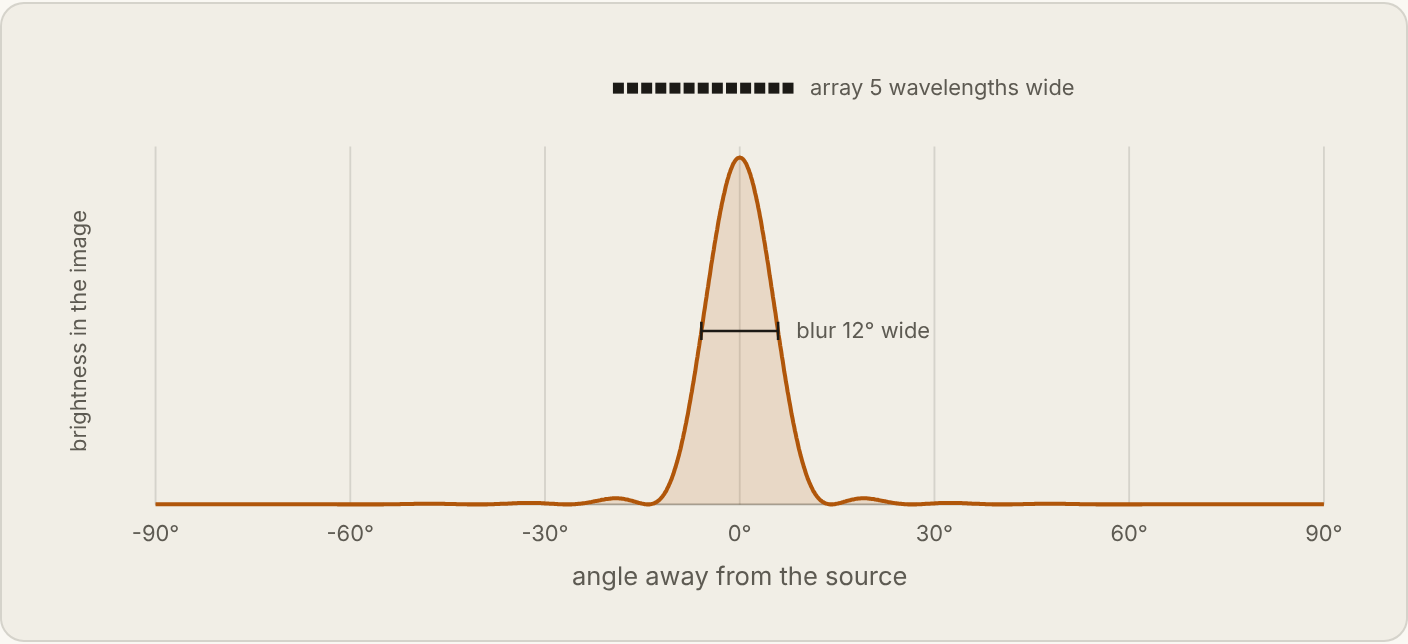
\includegraphics[width=\linewidth]{figures/array.png}
\caption{How sharply a camera can tell directions apart. The curve is the
response to a single distant source as the computed image is steered away from
it. A single pixel is not blind to direction, but its view of the sky is
blurred over tens of degrees. An array sharpens in proportion to its width in
wavelengths, Eq.~\eqref{eq:diffraction}.}\label{fig:array}
\end{figure}

\paragraph{What one pixel knows.} A single LIGO cannot tell where a wave came
from. A single ideal pixel can do better, because it records all ten
components of the field. For a single wave, the tensors $\tE_{ij}$ and
$\tB_{ij}$ together fix the direction of travel. For a sky full of independent
sources the pixel's data determine the brightness of the sky only in its
broadest patterns: those of spherical-harmonic degree four or less,
twenty-five numbers in all. It is the gravitational counterpart of the
statement that a single antenna has a broad beam, and it is the precise sense
in which one pixel is not yet a camera.

The proof is short. Independent waves add their second moments, so the
pixel's data are integrals over the sky of the brightness $I(\hat n)$ and the
circular polarization $V(\hat n)$ against kernels made from the polarization
tensors of a plane wave travelling along $\hat n$. For the brightness the
kernel is the sum over the two polarizations,
\begin{equation}\label{eq:pixel-kernel}
\sum_{A=+,\times} e^{A}_{ij}\, e^{A}_{kl}
= P_{ik}P_{jl} + P_{il}P_{jk} - P_{ij}P_{kl},
\qquad P_{ij} = \delta_{ij} - \hat n_i \hat n_j ,
\end{equation}
a polynomial of degree four in the components of $\hat n$; the kernel for $V$
is the antisymmetric combination, also a polynomial of degree at most four.
A polynomial of degree four on the sphere contains spherical harmonics of
degree four and below only, so by their orthogonality every harmonic of $I$
and $V$ above degree four integrates to zero. The magnetic tensor of a plane
wave is the electric one turned by $45^\circ$ about $\hat n$, so the same
holds for every product of $\tE$ and $\tB$. The linear polarization carries
spin weight four about $\hat n$ and enters only through its harmonic of degree
exactly four. The reference implementation checks all three statements
numerically, harmonic by harmonic.

\section{Telling waves from pull, and seeing in depth}\label{sec:separation}

\begin{quote}
\textbf{In plain words.} A wave from far away arrives at every pixel of the
camera almost identically, and so, nearly, does the pull of anything that is
not very close. What gives the wave away is its other half: a wave twists
spacetime as strongly as it stretches it, while still matter only stretches.
Nearby objects pull differently on different pixels, and those differences
tell how far away each thing is.
\end{quote}

Section~\ref{sec:pixel} ended with a difficulty: from the electric part alone,
one pixel cannot tell a wave from the pull of a passing lorry. With all ten
numbers it can (Section~\ref{sec:one-pixel}), and an array can do much more.
Three properties separate the two kinds of field.

\paragraph{Shape.} A plane wave stretches and squeezes only across its
direction of travel, so its tidal tensor has one vanishing eigenvalue and
$\det\tE = 0$. The field of a single mass has eigenvalues in the ratio
$-2 : 1 : 1$, and its determinant is never zero. One reading of one pixel
therefore distinguishes a single wave from a single mass. The test is for an
isolated source: the fields of several masses, or of several waves, add, and
their sum can have either form. The complex matrix of
Section~\ref{sec:one-pixel} goes further: a pure wave has
$\mathrm{tr}\,\mathcal{W}^2 = \mathrm{tr}\,\mathcal{W}^3 = 0$, two crossing waves have
$\det\mathcal{W} = 0$, and any single body has a repeated eigenvalue.

\paragraph{The magnetic part.} In a wave the magnetic tidal tensor is as large
as the electric one; it is the same pattern turned by $45^\circ$ about the
direction of travel. Near slowly moving matter it is smaller by the ratio of
the matter's speed to that of light,
\begin{equation}\label{eq:magnetic-ratio}
\frac{|\tB|}{|\tE|} = 1 \quad\text{(wave)},
\qquad
\frac{|\tB|}{|\tE|} \sim \frac{v}{c} \quad\text{(near field)} ,
\end{equation}
where $|\tE|^2 = \tE_{ij}\tE_{ij}$ (the Frobenius norm) and likewise for $\tB$,
and $v$ is the speed of the matter. At a distance $r$ from a compact source of
size $L$, the part of the field that changes is smaller by about $(v/c)(r/L)$,
that is, by $kr$ at the frequency of the change: more than $v/c$, but still far
below one in the near zone.
Averaged over time, the first holds for any mixture of waves from independent
sources, so the magnetic part is a detector of radiation that the pull of
nearby objects hardly touches. Coherent waves are an exception: in a standing
wave the magnetic part vanishes where the electric part is largest.

\paragraph{What the magnetic part sees nearby.} Small as it is, the near-field
magnetic tensor carries its own picture. To first order in $v/c$, a mass $M$ in
direction $\hat n$ at distance $r$, moving with velocity $\mathbf{v}$, gives
\begin{equation}\label{eq:magnetic-point}
\tB_{ij} = \frac{3GM}{c\,r^{3}}\,\bigl[\hat n_i(\hat n\times\mathbf{v})_j
+ \hat n_j(\hat n\times\mathbf{v})_i\bigr],
\end{equation}
which we have checked against the curvature of the metric of moving masses,
computed independently by finite differences. Grouping matter by direction
as in Eq.~\eqref{eq:tidal-column} gives the magnetic counterpart of the sky
integral,
\begin{equation}\label{eq:current-column}
\begin{gathered}
\tB_{ij} = \frac{3G}{c}\int\dd\Omega\,\bigl[\hat n_i(\hat n\times\mathbf{J})_j
+ \hat n_j(\hat n\times\mathbf{J})_i\bigr],\\
\mathbf{J}(\hat n) = \int \rho\,\mathbf{v}(r\hat n)\,\frac{\dd r}{r} ,
\end{gathered}
\end{equation}
so the magnetic half of the camera images the \emph{current column}
$\mathbf{J}$, with the same blur law at a signal-to-noise ratio smaller by
about $v/c$. Three things follow. Only motion across the line of sight counts:
$\hat n\times\mathbf{J}$ removes the radial part, so the magnetic channel is
the opposite of a Doppler radar, blind to approach and sensitive to sideways
motion. For a single moving mass $|\tB|/|\tE| = \sqrt3\,v_\perp/c$ to first order
in $v/c$, so one reading of one pixel gives the line on which a body lies (the
eigenvector of $\tE$'s negative eigenvalue, up to its sign) and, from $\tB$, its
sideways speed; at any speed, the four stars give the sideways velocity
exactly, Eq.~\eqref{eq:star-velocity}. And outside a spherical body spinning with angular momentum
$\mathbf{L}$ the field is exactly that of a spin dipole,
$\tB_{ij} = -(3G/cr^{4})[L_i\hat n_j + \hat n_iL_j
+ (\mathbf{L}\cdot\hat n)(\delta_{ij} - 5\hat n_i\hat n_j)]$: a hollow shell and
a solid ball of equal mass and size spinning at the same rate, whose electric
fields are identical everywhere outside them, differ in $\tB$ by their moments
of inertia, a factor $5/3$. At equal angular momentum they are identical
outside, and so motion too can hide. A uniform ball of radius $2^{-1/5}R$
turning one way inside a shell that reaches to $R$ and turns the other way at
the same rate has no angular momentum, and outside it no magnetic field at all,
though all of it moves; the reference implementation confirms the cancellation.
For a ball turning at angular velocity $\boldsymbol\omega$ about a point
$\mathbf{s}$, entered and left by the line of sight at distances $0 < a \le b$,
it is
$\mathbf{J} = \rho\,[(\boldsymbol\omega\times\hat n)(b-a)
- (\boldsymbol\omega\times\mathbf{s})\ln(b/a)]$. A smooth flywheel looks the
same spinning or still, and pulls the same; its current column is a vortex
that turns as the wheel turns. The demonstration of a sealed flywheel shows
it.

\paragraph{Variation across the array.} A wave of wavelength $\lambda$ changes
across an array of width $a$ by a fraction of order $2\pi a/\lambda$. The field
of a mass at distance $r$, which falls as $1/r^{3}$, changes by a fraction of
order $3a/r$. For a one-metre array, a wave at $100\,\mathrm{Hz}$ and a person
three metres away, these are $2\times10^{-6}$ and $1$. Subtracting the
average over the array therefore removes the wave and keeps the variation of
the neighbourhood. The reverse is harder: the average itself contains the pull
of everything nearby, and the person alone adds $3\times10^{-10}\,\mathrm{s^{-2}}$
to it, a million times the tidal field of the waves LIGO detects. To isolate
the wave the camera must model the nearby masses from their variation and
subtract them, which is how observatories plan to remove the changing pull of
their surroundings \cite{Harms2019,Chaibi2016}, or use the magnetic part, or
compare two arrays far apart; a camera simply keeps what the observatories
throw away. With two arrays far apart the separation is cleaner still: a wave
appears in both, with a delay that gives its direction, while a nearby mass
appears in one. The accompanying demonstrations show the tidal tensor itself
on a slice through the scene, coloured by the direction of stretching in the
manner of diffusion tensor imaging.

\paragraph{Depth.} The same variation measures distance. For an isolated mass
the tidal field goes as $M/r^{3}$ and its gradient as $M/r^{4}$, so their
ratio gives $r$, and then $M$: a pixel and its neighbours locate and weigh a
body with no need to move the camera. This is the principle by which a
calibration rotor's distance from a detector's mirror is found from the ratio
of two of its multipoles \cite{Inoue2018}. A single pixel can range a moving
mass without neighbours, but only with its magnetic part. The electric record
alone cannot do it: the record of a mass $M$ moving along $\mathbf{x}(t)$ is
unchanged if the path is enlarged $\lambda$-fold and the mass
$\lambda^3$-fold, while $\tB$ grows $\lambda$-fold, because the speed of light
supplies the scale. From Eq.~\eqref{eq:magnetic-point}, $\tB\hat n =
(3GM/cr^3)\,\hat n\times\mathbf v$ and $P\dot{\tE}\hat n = -(3GM/r^4)\,\mathbf
v_\perp$, with $P = 1 - \hat n\hat n$, so
\begin{equation}\label{eq:one-pixel-range}
r = c\,\frac{|\tB\hat n|}{|P\dot{\tE}\hat n|} ,
\end{equation}
and then $M$ from $\tE$; the sign that makes $r$ positive also fixes the sign
of $\hat n$. The reference implementation recovers distance, mass and velocity
this way from the finite-difference curvature of a moving mass. Motion straight
toward or away from the pixel gives no range, though it gives the time of
arrival, Eq.~\eqref{eq:contact}; and the magnetic signal, smaller by $v/c$, sets
the noise. For waves, range comes from the curvature of the wavefront, which
across an array of width $D$ amounts to a phase of order one at the distance
$D^{2}/\lambda$; beyond it range is still measured, with a fractional error of
order $\lambda r/\mathcal{R}D^{2}$ at signal-to-noise ratio $\mathcal{R}$. A
single pixel also ranges a wave source, from how its field departs from that of
a plane wave, Eq.~\eqref{eq:helicity-split}.

\paragraph{Front and back.} A flat array that records only the normal
component $\tE_{zz}$ cannot tell a mass in front of it from the mirror image of
that mass behind it, because the two give the same $\tE_{zz}$ on the plane. The
shear components $\tE_{xz}$ and $\tE_{yz}$ change sign between the two, so the
full tensor separates the half-spaces: a camera with no housing to block
gravity can still ignore the photographer standing behind it.

\paragraph{Three dimensions.} The pixels need not lie in a plane. A closed
shell of pixels sees the whole sky at once and has no blind side; pixels
filling a volume sample the field itself, although, as long as they stay
outside the matter, the ambiguity of Section~\ref{sec:near-field} remains. And in the thermal regime the transparency of matter makes a
further thing possible. Each image is then a set of line integrals, exactly
the data of a medical tomograph. Images from several positions can be combined
into a true three-dimensional map of emissivity, with nothing hidden behind
anything else.

These statements follow from the fields of
%   Sections~\ref{sec:pixel}--\ref{sec:waves}; the estimates of how well each
%   separation works in the presence of noise are still to be made.
% The text below begins with that paragraph's first sentence, kept. With it in place, the item "how well waves can
% be separated from nearby pull in the presence of noise, and the limits of the three-dimensional reconstructions of
% Section~\ref{sec:separation};" of paper/sections/12-status.tex is done, and the promise in the paragraph "How
% precisely" of paper/sections/02b-one-pixel.tex ("it ranges a moving mass with the precision that
% Section~\ref{sec:separation} gives") is kept by Eq.~\eqref{eq:magnetic-range}.
% References: three new entries in paper/drafts/separation_noise.bib (Ross2021, Thompson1982, Reid1990), to be added
% to paper/refs.bib. Figure: paper/figures/separation-noise.pdf, drawn by paper/figures/fig_separation_noise.py.
% Every number: reference/gravcam/separation_noise.py (paper_numbers), checked in
% reference/tests/test_separation_noise.py (test_numbers_quoted_in_the_draft and the tests above it).
% New labels: eq:magnetic-range, eq:depth-bound, fig:separation-noise.

These statements follow from the fields of
Sections~\ref{sec:pixel}--\ref{sec:waves}. How well each works against noise
follows from the Cram\'er--Rao bounds of the same fields, which the reference
implementation computes and checks against fits to simulated noisy readings
(Fig.~\ref{fig:separation-noise}). Each of a pixel's ten numbers carries white
noise, and $\rho$ is the signal-to-noise ratio of a signal at one pixel:
$|\mathcal{W}|/\sigma$ for one reading, as in Section~\ref{sec:one-pixel}, added
in quadrature over a record.

\paragraph{Separation with noise.} Take a wave at $100\,\mathrm{Hz}$ of strain
$10^{-21}$ and, $3\,\mathrm{m}$ from the camera, a rotor of two
$1\,\mathrm{kg}$ masses $12\,\mathrm{cm}$ apart turning 50 times a second,
about the quadrupole of the rotor that calibrates LIGO by its pull
\cite{Ross2021}. Its changing tide has the wave's frequency and a hundred times
its size. Shape alone tells an isolated wave from an isolated mass: the nearest
wave to the field of a mass, and the nearest mass to a wave, lie at half the
reading's size, so one reading of $\tE$ puts the two $\rho/2$ standard
deviations apart, and at $\rho = 12$ fewer than one reading in a hundred is
taken for the other. A wave and a near field together are separated by the
magnetic part, at a fixed price. Let the near field's $\tE$ at the wave's
frequency be anything at all, and its $\tB$ below the noise. Fitting both then
enlarges the error of the wave's amplitude by exactly $\sqrt2$, however strong
the near field: the near field takes the wave's $\tE$, and the wave is read from
its $\tB$, which carries half its signal. The wave is seen at $\rho/\sqrt2$, and
the near field pays the same $\sqrt2$ in the two components it shares with the
wave and nothing in the other three. Ignored, the rotor would be read as a wave
35 times the true one. Its own magnetic part leaks less than $10^{-4}$ of the
wave, because the $\tB$ of a changing source in the near zone is smaller than
its $\tE$ by a factor of order $kr$, here $2\times10^{-6}$, not by $v/c$. An
array that reads only $\tE$ must instead model the rotor from its variation,
here as a point quadrupole of unknown moment and position. For a pixel and six
neighbours at distance $b$ along three axes, the cost $D$, the factor on the
wave's error, grows as $r/b$, because a quadrupole's tide falls as $r^{-5}$ and
its share of the centre's reading must be inferred from a variation smaller by
about $5b/r$. For $b \ll r$, $D$ lies between $0.22\,r/b$ and $0.55\,r/b$ over
orientations. For the rotor and an array one metre across, $b = 0.5\,\mathrm{m}$,
$D = 2.2$; the array overtakes the magnetic part beyond $b = 0.29\,r$, and with
both $D = 1.26$. In return the wave costs the rotor's moment and position
factors of 1.5 and 1.3 from $\tE$ alone, and 1.07 and 1.04 with $\tB$ too.
Modelling the rotor as a point leaves a false wave of $0.005$ of the true one,
from its next multipole, which matters only above $\rho \approx 270$; ignored,
the rotor would be read as 70 times the wave.

\paragraph{How well depth is measured.} For one mass the field and its gradient
give the range exactly, $r = \sqrt{15}\,|\tE|/|\nabla\tE|$ with norms over all
components, and the Cram\'er--Rao bounds on range and mass are
\begin{equation}\label{eq:depth-bound}
\Bigl(\frac{\sigma_r}{r}\Bigr)^2 = \frac{1}{\rho_E^2} + \frac{1}{\rho_G^2},
\qquad
\Bigl(\frac{\sigma_M}{M}\Bigr)^2 = \frac{16}{\rho_E^2} + \frac{9}{\rho_G^2},
\end{equation}
where $\rho_E$ and $\rho_G$ are the signal-to-noise ratios of the field and of
its gradient, whatever the direction. A pixel with six neighbours at distance
$b \ll r$ has $\rho_E = \sqrt7\,\rho$ and $\rho_G = \sqrt{30}\,\rho\,b/r$, so
$\sigma_r/r \approx r/(\sqrt{30}\,\rho b)$; wider, the curvature of the field
across the pixels helps further. For a person $3\,\mathrm{m}$ away and
neighbours $0.5\,\mathrm{m}$ out, $\sigma_r/r$ is between $0.90/\rho$ and
$1.08/\rho$, depending on direction, against $1.16/\rho$ from the closed form
(Fig.~\ref{fig:separation-noise}b). Both uses of the
variation rest on Euler's relation for a field homogeneous of degree $-N$ about
its source, $(\mathbf{x}_s - \mathbf{x})\cdot\nabla f = N f$, with $N = 3$ for
the tide of a mass and $5$ for a quadrupole, by which geophysicists find the
depth of buried sources from measured gradients \cite{Thompson1982,Reid1990}.
The magnetic part of one pixel, Eq.~\eqref{eq:one-pixel-range}, ranges a moving
mass with no neighbours to
\begin{equation}\label{eq:magnetic-range}
\frac{\sigma_r}{r} = \frac{1}{\rho_B} ,
\end{equation}
$\rho_B$ the signal-to-noise ratio of $\tB$ alone, $\sqrt3\,v_\perp/c$ times
that of $\tE$ in each reading: for a person walking at
$1.4\,\mathrm{m\,s^{-1}}$, $\sigma_r/r = 1.2\times10^{8}/\rho$, a hundred
million times worse than with neighbours. Depth along one line is the limit.
For bodies on one line through the pixel every derivative of $\tE$ there has the
pattern of a single mass, so field and gradient see one body at
$r_{\mathrm{eff}} = \sum_i M_i r_i^{-3} / \sum_i M_i r_i^{-4}$, weighted toward
the nearer: two equal masses $\Delta$ apart appear as one at
$r - \Delta^2/r$, and a rod of length $L$ pointing at the camera as a point
$L^2/3r$ nearer than its centre. The spread $s$ of the depths shows first in
the second derivatives, as a share $s^2/r^2$ of them, which the seven pixels
read to $1/\rho_H$, with $\rho_H$ between $8.1$ and $10.5$ times
$\rho\,(b/r)^2$ depending on direction. Two equal masses, $s = \Delta/2$, are
therefore told from one only when $\Delta > 2r/\rho_H^{1/2}$, between $0.62$
and $0.70$ times $(r^2/b)/\rho^{1/2}$: the square-root law that
Section~\ref{sec:near-field} found for masses side by side. A round body of any
size is a point, and its size is not measured at all.

\begin{figure*}
\centering
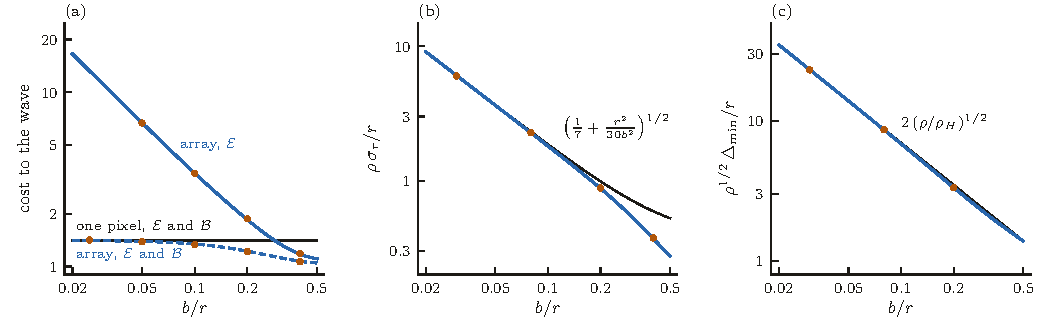
\includegraphics[width=\textwidth]{figures/separation-noise.pdf}
\caption{Separation and depth with noise, against the distance $b$ of a pixel's
six neighbours over the distance $r$ of the source. Blue: Cram\'er--Rao bounds
of the full models; black: closed forms; dots: the spread of
maximum-likelihood fits to simulated noisy readings. (a) The factor $D$ by
which fitting the rotor of the text enlarges the error of a wave's amplitude:
at one pixel from $\tE$ and $\tB$, with any near field, $\sqrt2$ (the dot at
left is a simulation with the rotor present); for the array, which fits the
rotor as a point quadrupole of unknown moment and position, from $\tE$ alone
(solid) and from both (dashed). (b) The range of one mass, with $\rho$ the
signal-to-noise ratio of one pixel's reading, against
Eq.~\eqref{eq:depth-bound}. (c) The separation $\Delta_{\min}$ in depth at which
two equal masses on one line are told from one at one standard deviation.
Computed in the reference implementation.}\label{fig:separation-noise}
\end{figure*}

\section{A first image}\label{sec:first-image}

Because nothing absorbs or scatters, a thermal gravitational image is a line
integral. Integrating Eq.~\eqref{eq:kirchhoff} over frequency for constant
$\eta$ gives the energy emitted per unit volume and solid angle,
$j_E = \alpha\sigma T^4/\pi$, where $\sigma$ is the Stefan--Boltzmann constant.
Dividing by the mean energy of a thermal quantum, $2.70\,\kB T$, gives a
number emissivity $j_N$, and the brightness of the pixel that looks along the
unit vector $\hat n$ is
\begin{equation}\label{eq:column}
N(\hat n) = \int_0^\infty j_N\bigl(s\,\hat n\bigr)\,\dd s ,
\end{equation}
in gravitons per second, per square metre of aperture, per steradian.

Figure~\ref{fig:sun-at-midnight} evaluates Eq.~\eqref{eq:column} for an
observer on the night side of the Earth, at latitude $40^\circ$ at local
midnight. The Earth is modelled as five uniform shells with rounded textbook
radii and temperatures, from a crust at $700\,\mathrm{K}$ to an inner core at
$5500\,\mathrm{K}$. Looking straight down, the line of sight runs through
$12{,}700\,\mathrm{km}$ of rock and iron, and the expected brightness is
$6\times10^{-5}$ gravitons per second per square metre per steradian. The
Sun radiates of order $10^{8}\,\mathrm{W}$ in gravitational waves
\cite{GarciaCelyRingwald2025,Steane2024}, about
$4\times10^{-16}\,\mathrm{W\,m^{-2}}$ at the Earth: roughly one graviton per
square metre per second, arriving from a patch of sky a tenth of a degree
across. Its surface brightness is some $10^{10}$ times that of the Earth's
interior in this model, so the Sun dominates the thermal gravitational sky by
day and by night.

Two assumptions carry most of the uncertainty. The Earth's internal friction
at thermal frequencies is not known to us, and is set to
$\eta = 10^{-3}\,\mathrm{Pa\,s}$ throughout as a placeholder. The Sun's
emission is spread uniformly over the inner fifth of its radius, where the
true profile is peaked toward the centre.

\paragraph{How faint.} The image is an expectation value. Figure~\ref{fig:budget}
sets the numbers of gravitons emitted side by side, and Table~\ref{tab:budget}
the numbers a camera would receive in each of the accompanying demonstrations.
The Sun delivers about one graviton per square metre per second. The whole
Earth below, in this model, delivers one every five hours, about $10^{5}$ per
square metre in a lifetime: enough for a coarse picture of the planet's
interior, if the assumed friction is right. Everyday objects in a room take
millions of years for a single graviton.

\begin{table}
\centering
\begin{tabular}{p{0.42\linewidth}p{0.22\linewidth}p{0.26\linewidth}}
Demonstration, and what is counted & Regime & One graviton per square metre every \\ \hline
The Sun at midnight: the Sun's core & thermal & second \\
The Sun at midnight: the whole Earth below & thermal & 5 hours \\
Honey and water: the honey, at $2\,\mathrm{m}$ & thermal & $10^{6}$ years \\
The closed furnace: the hot iron, at $3.5\,\mathrm{m}$ & thermal & $2\times10^{7}$ years \\
Which way it turns: one turning pair, at $4.5\,\mathrm{m}$ & waves & $4\times10^{7}$ years \\
The other demonstrations & near field & none needed \\
\end{tabular}
\caption{The graviton budget of the demonstrations, for a detector of one
square metre, from the reference implementation. Thermal rates scale with the
assumed internal friction. The near field is a static field, not radiation:
what limits it is noise, Eq.~\eqref{eq:resolution}, not the number of
gravitons.}\label{tab:budget}
\end{table}

\begin{figure}
\centering
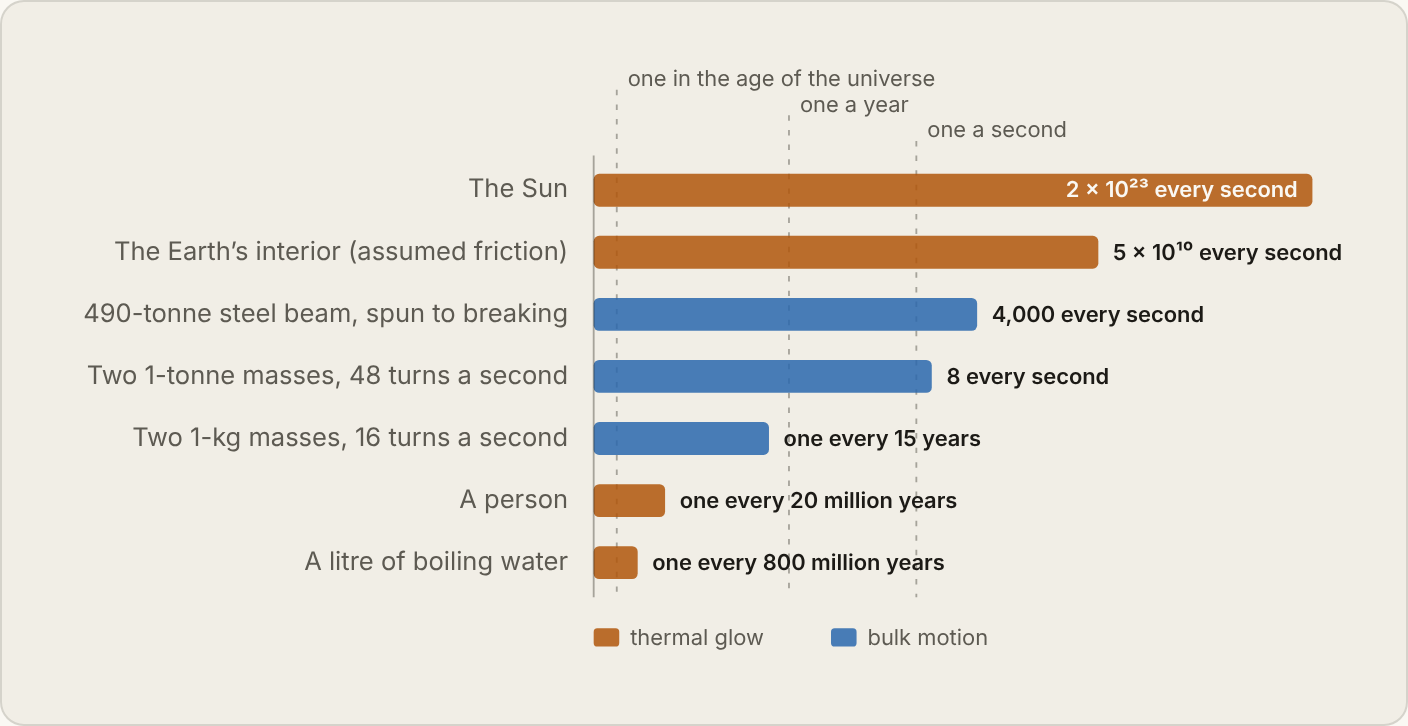
\includegraphics[width=\linewidth]{figures/budget.png}
\caption{Gravitons emitted per second by whole objects, on a logarithmic
scale spanning forty powers of ten. The spinning masses radiate by bulk
motion, Eq.~\eqref{eq:dumbbell}; the others thermally,
Eq.~\eqref{eq:kirchhoff}, with a constant friction that makes the thermal
values upper estimates. The Earth's value depends on its assumed
friction.}\label{fig:budget}
\end{figure}

All images shown with this paper are computed twice: by the engine that draws
them, and by an independent reference implementation that integrates
Eq.~\eqref{eq:column} by a different method. The two agree to a few parts in a
million along ordinary lines of sight.

\section{What the camera can do that light cannot}\label{sec:affordances}

Table~\ref{tab:affordances} collects what follows from the preceding sections
for someone holding the camera. Each line corresponds to a demonstration on
the accompanying site, in which one half of the picture is taken in light and
the other in gravity.

\begin{table}
\begin{tabular}{p{0.26\linewidth}p{0.4\linewidth}p{0.22\linewidth}}
The camera can & Because & Regime \\ \hline
See through anything & nothing absorbs or scatters gravity & near field, thermal \\
Find what is hidden & mass has one sign, so no shield or cloak exists & near field \\
Weigh by looking & the signal is set by mass, not by surface & near field \\
Ignore images & a mirror's reflection or a screen's picture has no mass & all \\
Read inside temperature & hot bodies are transparent to their own glow & thermal \\
Tell materials by their friction & emission follows internal friction & thermal \\
Read spin and its sense & polarization follows the motion of the source & waves \\
See flow inside a sealed body & the magnetic part of the field is made by moving mass & near field \\
See what emits no light & all energy gravitates & near field \\
\end{tabular}
\caption{What a gravitational camera affords, and why.}\label{tab:affordances}
\end{table}

The last line of the table includes light itself. A beam of power $P$ carries
energy and an equal pressure along its length, and to a static observer beside
it both gravitate: it pulls like a line of matter of $2P/c^{3}$ per metre,
twice what its energy alone would suggest \cite{TolmanEhrenfestPodolsky1931}.
An infrared beam that no camera can see from the side is, for this one, a
faint line; for a $100\,\mathrm{kW}$ beam, a change of one part in $10^{22}$
of the pull of the room around it, visible only by subtracting the reading
with the beam off.

The same reasoning tells what the camera cannot do. It cannot read a page,
recognise a face by its colouring, or see a picture on a screen: everything
that light carries by reflection from surfaces is absent. The two kinds of
camera are complementary, and a scene is best understood with both.

\section{Vistas}\label{sec:vistas}

\begin{quote}
\textbf{In plain words.} The same rules, applied to the sky. Close to a pair of
black holes the camera would see them as two, turning; farther out it sees
only the spiral of their waves. An exploding star is invisible unless it is
lopsided, and then it leaves space permanently stretched. The Milky Way's
centre, hidden from light behind dust, is the brightest thing in the
gravitational sky. And if the Big Bang was ever hot enough, the whole sky
glows at a temperature just under one kelvin, a background against which the
only shadows are black holes.
\end{quote}

The scenes so far are rooms and planets. This section follows the same
equations to the scales where they are most striking. We chose problems that
have exact or closed-form solutions, so that every picture below is computed
from physics, not drawn; each is checked by tests in the reference
implementation. The website lets the reader look around three of these skies
live.

\paragraph{A pair of black holes, from the inside out.} Outside any compact
source, linearized gravity has an exact solution organised by multipoles
\cite{Thorne1980}. Kept to the order of the mass quadrupole $I_{ij}$, with
$u = t - r/c$ and $\hat n$ the direction from the source, the trace-reversed
perturbation in harmonic gauge is
\begin{equation}\label{eq:multipole}
\begin{aligned}
\bar h^{00} &= \frac{4G}{c^2}\Bigl[\frac{M}{r} + \frac{1}{2}\,\partial_i\partial_j\frac{I_{ij}(u)}{r}\Bigr],\\
\bar h^{0i} &= \frac{2G}{c^3}\Bigl[\frac{\dot I_{ij}(u)\,\hat n_j}{r^2} + \frac{\ddot I_{ij}(u)\,\hat n_j}{c\,r}
+ \frac{(\mathbf J\times\mathbf x)_i}{r^3}\Bigr],\\
\bar h^{ij} &= \frac{2G}{c^4}\,\frac{\ddot I_{ij}(u)}{r},
\end{aligned}
\end{equation}
with $M$ the mass, $\mathbf J$ the angular momentum and $I_{ij} = \int\rho\,
x_ix_j\,\dd^3x$ the second moment of the mass, its trace included (outside
the source the trace changes only the gauge, not the curvature, as the
reference implementation confirms). It satisfies the gauge condition exactly,
and its curvature gives the tidal field in every zone at once
\cite{Teukolsky1982}: exactly, within linearized gravity and this truncation
of the multipoles. Figure~\ref{fig:binary-field} shows it in the plane
of an orbit, for two black holes of thirty solar masses each about ten seconds
before they merge, when they are $2200\,\mathrm{km}$ apart and move at a tenth
of the speed of light; their waves are $35{,}000\,\mathrm{km}$ long. Within a
reduced wavelength, $\lambda/2\pi$, the changing part of the field is Newton's
pull of two masses, turning rigidly with them and falling as $r^{-5}$. Beyond
it the pattern winds into a two-armed spiral whose strength falls only as
$r^{-1}$: the waves. The two meet where
$G\,\Delta I/r^5 \approx G\,\Delta I\,\omega^4/c^4 r$, that is at
$r \approx c/\omega = \lambda/2\pi$.

This marks a crossover between the two ways the camera sees, not a sharp
edge. Well inside it the near-field imaging of Section~\ref{sec:near-field}
applies, and an array could resolve the pair as two bodies, if its
signal-to-noise ratio and width meet the blur law there; well outside it,
Eq.~\eqref{eq:unresolved} holds and the pair is a point whose polarization
tells the axis and sense of its orbit. Being within about a sixth of a
wavelength is needed to see two black holes as two, but it is not enough by
itself. The reference
implementation computes the field of Eq.~\eqref{eq:multipole} by finite
differences of the curvature and checks that it becomes Newton's field of the
two masses near them, with an error falling as $(d/r)^2$, and the quadrupole
wave far away, with an error falling as $\lambda/r$, and that it is the
curvature of vacuum, with $|\tB| = |\tE|$ in the waves.

\begin{figure*}
\centering
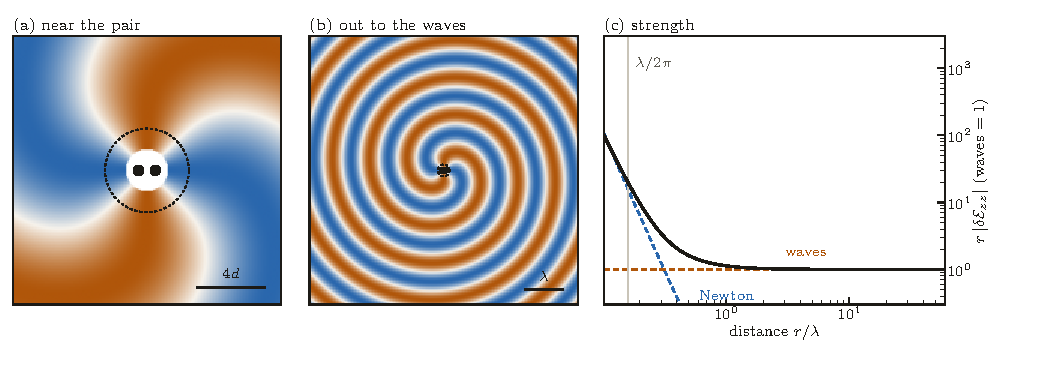
\includegraphics[width=\textwidth]{figures/binary-field.pdf}
\caption{Two black holes of thirty solar masses, ten seconds before they
merge, in the plane of their orbit: the changing part of the tidal field
$\tE_{zz}$ (across the plane), from the linearized solution of
Eq.~\eqref{eq:multipole}, exact within that model. Colour gives the phase, orange for stretch and blue
for squeeze, scaled at each place by the local strength. (a) Near the pair,
whose separation is $d$, the pattern turns rigidly with it; beyond the dashed
circle, $r = \lambda/2\pi$, it begins to wind. (b) Farther out it is the spiral
of the waves. (c) The strength along a line in the plane, times $r$: Newton's
$r^{-5}$ inside $\lambda/2\pi$, the waves' $r^{-1}$ outside. The field is an
exact solution of linearized gravity truncated at the mass quadrupole, which
this close to a merger is a guide to the full solution, not a substitute for
it.}\label{fig:binary-field}
\end{figure*}

\paragraph{What a burst leaves behind.} Radiation that escapes to infinity
carries away mass, and a camera it passes is left permanently deformed: the
memory \cite{Christodoulou1991,Thorne1992}. For energy radiated with angular
distribution $\dd E/\dd\Omega'$, at nearly the speed of light, the change in
strain seen from direction $\hat N$ at distance $r$ is
\cite{Epstein1978,Thorne1992}
\begin{equation}\label{eq:memory}
\Delta h_{ij}^{\TT} = \frac{4G}{c^4 r}\int \frac{\dd E}{\dd\Omega'}
\left[\frac{n'_i n'_j}{1 - \hat n'\cdot\hat N}\right]^{\TT}\dd\Omega' .
\end{equation}
Applied to the waves of a merger themselves, whose power goes as
$(1+\cos^2\iota)^2/4 + \cos^2\iota$, it gives
\begin{equation}\label{eq:merger-memory}
\Delta h_+ = \frac{G\,\Delta E}{24\,c^4 r}\,\sin^2\iota\,\bigl(17 + \cos^2\iota\bigr),
\end{equation}
the shape found by Wiseman and Will \cite{WisemanWill1991,Favata2009}, which
we reproduce by integrating Eq.~\eqref{eq:memory} numerically. It is largest
seen edge-on, where the oscillating wave is weakest (Figure~\ref{fig:memory}).
A camera that records the field, not the strain, sees the memory as a burst of
$\tE$ whose second time integral does not return to zero.

\paragraph{An exploding star.} A spherical collapse or explosion radiates
nothing: by Birkhoff's theorem the field outside a spherical body is that of a
point mass, whatever happens within. It does change once. A core collapse
sends out some $3\times10^{46}\,\mathrm{J}$ in neutrinos, a sixth of a solar
mass, as a thin shell moving at nearly the speed of light, and outside the
shell the field is that of the original mass, inside it that of the remnant
\cite{Vaidya1951}. A near-field camera sees the star lose the neutrinos'
mass at the moment the shell passes the camera, not before: it weighs the
burst as it arrives. While the shell passes, the camera also feels the
neutrinos themselves. Their flux of energy, $F = L/4\pi r^2$ at luminosity
$L$, enters the Ricci part of the curvature and squeezes the camera evenly
across their direction of travel, $\tE_{ij} = (GL/c^3r^2)(\delta_{ij} - \hat
n_i\hat n_j)$, while $\tB$ gains the antisymmetric part of
Section~\ref{sec:pixel}, set by their flow, so that one pixel points to the
star although the explosion is spherical. From ten kiloparsecs this squeeze,
while it lasts, is some $10^{11}$ times the change of pull it leaves behind. If the neutrinos leave unevenly the explosion also leaves
memory \cite{Epstein1978,Turner1978}. A narrow jet of energy $E$ leaves
$\Delta h = (2GE/c^4 r)(1 + \cos\theta)$ at angle $\theta$ from it, largest
just off the line it travels along (exactly on that line symmetry allows
none, and a jet of finite width turns the memory off within its own width
of the axis); two opposite jets leave the same $2GE/c^4 r$ in every
direction off their axis; a sphere leaves nothing (Figure~\ref{fig:memory}).
Only the quadrupole and higher parts of the pattern count: the radiation of a
burst that is merely brighter on one side, a pure dipole, leaves no memory at
all. It does push the star the other way, and the recoiling remnant leaves a
memory of its own, second order in the small recoil \cite{Favata2009}. A burst
stronger along an axis than across it, in proportion to
$1 + q\,P_2(\cos\theta')$, leaves
\begin{equation}\label{eq:burst-memory}
\Delta h = \frac{q\,G E}{2\,c^4 r}\,\sin^2\theta .
\end{equation}
For a supernova ten kiloparsecs away and $q = 0.01$ this is
$4\times10^{-21}$ seen from the side.

\begin{figure}
\centering
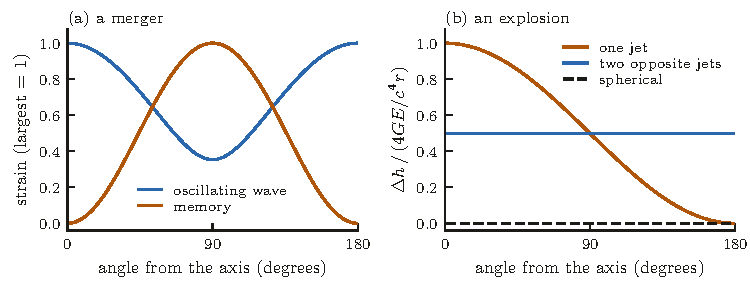
\includegraphics[width=\columnwidth]{figures/memory.pdf}
\caption{The memory, Eq.~\eqref{eq:memory}, against the direction of the
camera. (a) A merger: the oscillating wave is strongest along the orbit's
axis, the memory, Eq.~\eqref{eq:merger-memory}, in its plane. (b) An
explosion whose energy leaves in one jet, in two opposite jets, or evenly in
all directions, in units of $4GE/c^4 r$.}\label{fig:memory}
\end{figure}

\paragraph{The Milky Way.} Tens of millions of close pairs of white dwarfs
radiate at millihertz frequencies; together they make a foreground that will
dominate the sky of the planned space detectors below a few millihertz
\cite{Nelemans2001}. They trace the Galaxy's stars, and averaged over time
and over orientations, which we take to be random, each radiates the same in
every direction; so their brightness on the sky is the column integral of
Eq.~\eqref{eq:column} over a model of the stellar mass, here two exponential discs and a central bulge with masses and
sizes from Bland-Hawthorn and Gerhard \cite{BlandHawthornGerhard2016}. Light
from the same stars passes through a thin disc of dust, which in this model
dims the light of the Galactic centre by about forty magnitudes, comparable
with what is observed. Figure~\ref{fig:milky-way}
shows both on one scale. In light the centre is hardly brighter than the opposite
side of the sky; in gravitational waves it is a hundred times brighter, and
the map is a map of where the Galaxy's stars are. Seeing it this sharply as
a smooth glow would take a camera some $50\,\mathrm{AU}$ across, since at three
millihertz the waves are two-thirds of an astronomical unit long. The pairs are
not a glow, though: after years of observation thousands of the brightest,
above a few millihertz, would each sit alone in its own frequency bin, and a
single pixel could place each of them by Eq.~\eqref{eq:one-wave}, breaking the
smooth map into points.

\begin{figure}
\centering
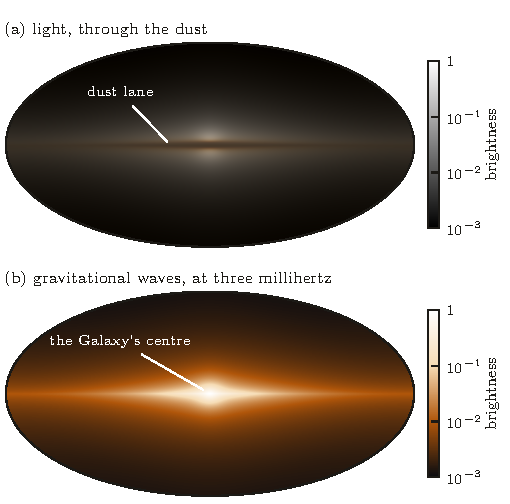
\includegraphics[width=\columnwidth]{figures/milky-way.pdf}
\caption{The Milky Way from the Sun, over the whole sky, centred on the
Galaxy's centre with longitude increasing to the left, both on one logarithmic
scale of brightness. (a) Light from the model's stars, dimmed and reddened by
its dust. (b) Gravitational waves from white-dwarf pairs that trace the same
stars, as an ideal camera about $50\,\mathrm{AU}$ across would see them at
three millihertz. Without its dust, (a) would be identical to (b) in
brightness.}\label{fig:milky-way}
\end{figure}

\paragraph{The first light.} Gravitons stop interacting near the Planck
temperature. If the early universe was ever that hot, they were then in
equilibrium and have kept a black-body spectrum ever since. Every species that
later annihilated heated the photons but not them, so by conservation of
entropy their temperature today is \cite{KolbTurner1990}
\begin{equation}\label{eq:graviton-temperature}
T_g = \left(\frac{3.91}{106.75}\right)^{1/3} T_{\gamma} = 0.905\,\mathrm{K},
\end{equation}
with $T_\gamma = 2.7255\,\mathrm{K}$ \cite{Fixsen2009} and the particles of the
Standard Model; more particles would make it colder. Whether this background
exists is a test of inflation, which would have diluted it away
\cite{VagnozziLoeb2022}. Its energy density counts as $0.05$ of an extra
species of neutrino, within present bounds.

If it exists, it carries more energy than any other background in the
gravitational sky: $7\times10^{-7}$ of the critical density, against about
$10^{-8}$ for the background found by pulsar timing at nanohertz frequencies
\cite{NANOGrav2023}. At high frequencies it outshines everything else in this
paper. A black body of two polarizations sends
$N = 4\zeta(3)(k_BT/h)^3/c^2$ quanta per second per square metre per
steradian: $3.6\times10^{14}$ at $0.905\,\mathrm{K}$, against $6\times10^{-5}$
for the Earth's interior and $4\times10^{5}$ for the Sun's core
(Section~\ref{sec:first-image}). It is also the easiest to image. Its
gravitons are about a centimetre long, so an aperture of a metre resolves a
degree. Four properties follow from what is already known.
\begin{itemize}
\item \emph{It moves with us.} Our motion through it at $370\,\mathrm{km/s}$
\cite{Planck2018I} makes one side of the sky hotter by $v/c = 1.2\times10^{-3}$
of its temperature, exactly as for the microwave background.
\item \emph{On large scales it shares the microwave background's spots.} On scales larger
than the horizon at the time the microwave background was released, the
Boltzmann equation of any massless species reduces to
$\dot\Theta = -\dot\Phi$ ($\Theta$ the fractional change of temperature, $\Phi$ that of the spatial metric), the same for gravitons streaming freely as for
photons held in the plasma. With the same adiabatic start, the two arrive at
that time with the same temperature perturbation, and from then on travel
together through the same potentials. To this approximation the graviton sky
shares the large spots of the microwave sky, from a surface only $2\%$
farther away; how closely, scale by scale, is a question for a
cross-correlation of the two. It differs below a degree or so, where it has no
acoustic peaks, its gravitons never having moved with the plasma, and it is
not smoothed by the diffusion that blurs the microwave sky below a few
arcminutes, since its gravitons never scattered \cite{Bartolo2019}.
\item \emph{Lensing leaves its uniform part unchanged.} Bending conserves
surface brightness, so a uniform background stays uniform however its rays are
bent; only its departures from uniformity, the dipole of our motion and the
spots, are moved about.
\item \emph{Only black holes cast shadows on it.} Nothing else absorbs
appreciably across a broad band (Section~\ref{sec:no-lens}). Seen against this background, the sky is a
uniform glow at $0.905\,\mathrm{K}$, warmer in the direction of our motion,
with a black disc wherever a black hole stands.
\end{itemize}
Figure~\ref{fig:black-hole} computes one such view by exact rays of the
Schwarzschild metric \cite{Darwin1959,Synge1966,Luminet1979}. The camera is at
rest $40\,GM/c^2$ from a black hole that lies just above the Galaxy's centre.
In light, the Milky Way bends around the hole into a ring, with a second image
above it. In primordial gravitons the background is uniform except for the
dipole of our motion, so all that shows is the shadow, of angular radius
$\sin^{-1}[\sqrt{27}\,(GM/c^2 r)\sqrt{1-2GM/c^2 r}] = 7.3^\circ$, and the
dipole folded around it. The whole sky is $2.6\%$ warmer than far from the
hole, $T_g/\sqrt{1-2GM/c^2 r}$, so the camera's thermometer also reads how deep
it sits in the hole's potential.

A black hole is dark against this background only because it is colder. Its
Hawking temperature, $\hbar c^3/8\pi GMk_B$, equals $0.905\,\mathrm{K}$ for a
mass of $1.36\times10^{23}\,\mathrm{kg}$, nearly two masses of the Moon. A
heavier hole casts a shadow; a lighter one glows against the sky; and one of
just this mass, in equilibrium with the background, returns in every mode
exactly what it receives and cannot be seen at all. Spin changes this too. A
spinning hole amplifies the waves that turn with it, by up to $138\%$ for the
most favoured mode of a hole spinning near its limit
\cite{TeukolskyPress1974}, so at wavelengths comparable to its size it would
return more of the background than it receives on that side, and appear
brighter than the sky there rather than dark.

Mode by mode the bookkeeping is exact. A wave of angular degree $l$ and
frequency $\omega$ that reaches the hole is absorbed with probability
$\Gamma_l(\omega)$ and otherwise scattered back, and the hole emits in the
same proportion, so what the camera receives from it in that mode differs
from the sky's occupation $n_{\mathrm{bg}}$ by $\Gamma_l\,(n_H - n_{\mathrm{bg}})$,
with $n_H$ the occupation at the hole's temperature. For a spinning hole
$n_H$ is taken at $\omega - m\Omega_H$, $\Omega_H$ the angular velocity of its
horizon, and in the modes that turn with it faster than it, $\omega <
m\Omega_H$, both factors change sign: whatever the temperatures, those modes
come out brighter than the sky. For a hole that does not spin we have computed
$\Gamma_l$ for every mode from the Regge--Wheeler equation. The shadow is then
less deep than the black disc of the geometric cross-section $27\pi G^2M^2/c^4$
suggests, because the sky's gravitons are not short compared with the hole:
against the $0.905\,\mathrm{K}$ background, a hole ten times the equilibrium
mass is $93\%$ as dark as that disc, three times, $60\%$, and twice, $29\%$;
only above about a hundred times, $10^{25}\,\mathrm{kg}$, is it black. The
reference implementation checks the conservation of flux in every mode,
Page's limit for long waves, $\Gamma_2 \to (256/225)(GM\omega/c^3)^6$
\cite{Page1976}, and the geometric cross-section for short ones.

\begin{figure*}
\centering
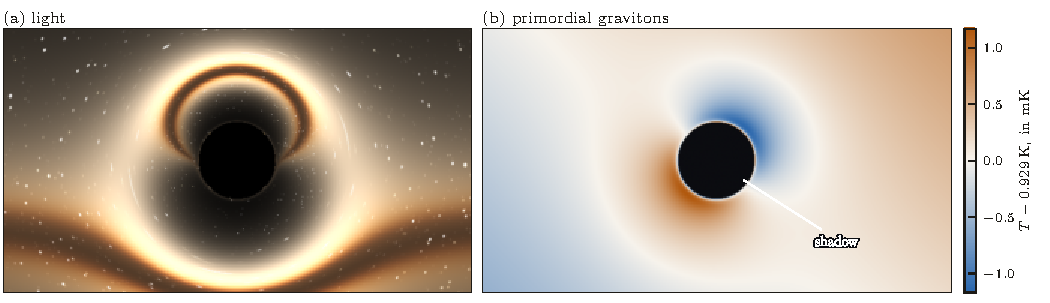
\includegraphics[width=\textwidth]{figures/black-hole.pdf}
\caption{A black hole seen from rest $40\,GM/c^2$ away, through exact
Schwarzschild rays, with the Galaxy's centre $9^\circ$ below the hole. (a) Light:
the model Milky Way of Figure~\ref{fig:milky-way}, with stars added for
orientation, bent into a ring around the shadow and a second image above it.
(b) The primordial graviton background, Eq.~\eqref{eq:graviton-temperature},
warmed to $0.929\,\mathrm{K}$ by the depth of the potential and hotter toward
our direction of motion; the colour shows its departure from the mean, folded
around the shadow by the bending. Nothing else in a gravitational image casts
a shadow.}\label{fig:black-hole}
\end{figure*}

\paragraph{The transparent Sun as a lens.} Gravitational waves pass through
the Sun and, where geometric optics holds, are bent by the mass inside the
cylinder of their impact parameter, $\alpha(b) = 4GM_{\mathrm{cyl}}(b)/c^2 b$.
For Eddington's standard model of the Sun the bending peaks at $4.2''$ for
rays passing $0.28$ of a radius from the centre, more than twice the
$1.75''$ of rays that graze it (Figure~\ref{fig:sun-lens}). Rays through the
centre come to a focus first, $c^2/4\pi G\Sigma(0) = 34\,\mathrm{AU}$ behind
the Sun, where $\Sigma$ is the column density; Patla and Nemiroff found
$23.5\,\mathrm{AU}$ for the denser core of the standard solar model
\cite{PatlaNemiroff2008}. From farther away a compact source directly behind
the Sun appears as a ring inside the solar disc, at the impact parameter
whose focus lies at the camera. A uniform background, such as the primordial
one, is not changed.

Geometric optics needs more than a wavelength shorter than the Sun. A lens of
mass $M$ delays a wave by about $4GM/c^3$, twenty microseconds for the Sun, and
it focuses only if that delay spans a radian or more of the wave's phase, that
is above $c^3/8\pi GM = 8\,\mathrm{kHz}$ for the Sun, whatever its size. Below,
diffraction erases the focus: even a point of the Sun's mass raises the
intensity on its axis only by the factor $\pi w/(1 - e^{-\pi w})$, with $w =
8\pi GMf/c^3$, which is $1.02$ at $100\,\mathrm{Hz}$. The transparent Sun is a
lens for thermal and primordial gravitons, not for the waves of orbiting or
merging bodies.

Wave optics joins the two regimes. For a source directly behind the Sun the
amplitude on the axis, a distance $d$ behind it, is the Fresnel integral over
the plane of the Sun of $e^{ik[b^2/2d - \Phi(b)]}$, where $\Phi' = \alpha$ is
the extra path through its field. Outside the disc $\Phi$ is a point mass's,
and that part of the integral is an incomplete gamma function; inside it is
smooth, and we integrate it numerically. On Earth's orbit the Sun never raises
the intensity by more than the $6\%$ of the central ray's geometric focusing,
$(1 - d/f_0)^{-2}$ with $f_0 = 33.7\,\mathrm{AU}$, which it reaches only above
about $10\,\mathrm{kHz}$. Beyond the central focus a ring of rays from inside
the Sun converges on the axis, and the gain there grows in proportion to the
frequency: at $50\,\mathrm{AU}$ it is $3.4$ at $10\,\mathrm{kHz}$, $44$ at
$100\,\mathrm{kHz}$ and $480$ at $1\,\mathrm{MHz}$, from $1.1$ to $1.25$
times that of a point of the Sun's mass, $\pi w$, and equal to it at
$550\,\mathrm{AU}$, where the converging rays graze the limb. At the
frequencies of thermal gravitons, near $10^{13}\,\mathrm{Hz}$, the same
proportion gives some $5\times10^{9}$. The reference implementation checks the
method against the point mass's closed form, and both limits: long waves,
which see only the Sun's whole mass, and short ones, which follow the rays.

\begin{figure}
\centering
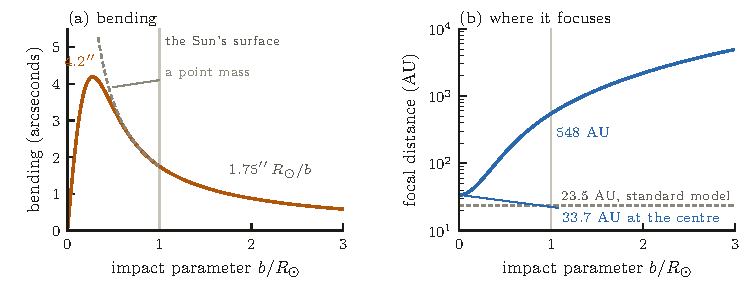
\includegraphics[width=\columnwidth]{figures/sun-lens.pdf}
\caption{The transparent Sun as a lens for gravitational waves, in
Eddington's standard model. (a) Bending against the impact parameter:
inside the Sun it rises to $4.2''$ and falls to zero at the centre; the dashed
curve is what a point mass would give. (b) The distance behind the Sun at
which the rays at each impact parameter cross the axis: $34\,\mathrm{AU}$
through the centre, $548\,\mathrm{AU}$ at the surface. The dashed line marks
the $23.5\,\mathrm{AU}$ found for the standard solar model.}\label{fig:sun-lens}
\end{figure}

\paragraph{Two further consequences.} There is no flash photography. To
light a scene and see what it reflects, matter would have to scatter
gravitational waves, and the cross-section of a body of mass $m$ is of order
$(Gm/c^2)^2$ \cite{Peters1976}, $10^{-50}\,\mathrm{m^2}$ for a person: every
picture in this paper is made by what the scene itself emits or how it pulls.
And an earthquake shows in two parts of the field. Compressional waves change
the density of the rock they cross, and with it $\tE$; that is the prompt
signal already recorded \cite{Vallee2017}. Shear waves in a uniform medium do
not change its density, but they move mass, and so appear in $\tB$, through
Eq.~\eqref{eq:current-column}.

\section{Open problems}\label{sec:status}

Six problems are open. Heat and an
applied tide fix a body's interior in principle, with no null space and through the
same logarithm as the static field (Section~\ref{sec:second-order}); how much of a real
body, the Earth for one, a finite record at finite sensitivity over a finite
band actually recovers has not been worked out. The pair of arrangements that
gravity cannot tell apart at one time, Eq.~\eqref{eq:dp-energy}, is a test of gravitational
collapse that is described here and not designed. The reading of a body by
an impulsive tide and a weighing, Eq.~\eqref{eq:push}, is exact in Newton's theory with
the weight of energy added, and for an impulsive plane wave it is
Eq.~\eqref{eq:shock}. A particle without mass that passes,
Eq.~\eqref{eq:massless-pass}, is the simplest wave sent in from infinity; the
statement for a general wave, with the mass read at infinity for the weight,
is a problem of scattering that has not been solved. The brackets of the
moments are given here to the first order in $1/c^2$,
Eq.~\eqref{eq:moment-bracket}; whether the moments of the full theory close
on a known algebra is open \cite{CompereOliveriSeraj2018}. The ceiling on
sensitivity of Section~\ref{sec:near-field} is a heuristic estimate; a bound
needs the coupling, the resources and the task to be stated exactly. And the
friction of real materials at the frequencies of heat, on which every thermal
count in this paper rests, deserves a microscopic calculation for at least one
crystal, phonon by phonon, of the kind already made for absorption by crystal
detectors \cite{KahnSchutteEngelTrickle2024}, and for the deep Earth at its
temperatures and pressures.

\section*{Use of AI}\label{sec:ai-use}

This work was carried out with Claude (Anthropic; the models Claude Opus 5.5
and Claude Fable 5.2), used throughout as a research assistant. Under the
author's direction it drafted and revised the text, carried out and checked
derivations, searched the literature and checked the references against their
sources, and wrote the reference implementation and its tests, the code that
draws the figures, and the interactive version of the scenes. The question,
the choice of problems and of what the paper says, and the judgment of the
results are the author's own; the author takes responsibility for every
statement in it. The pictured objects in Figs.~\ref{fig:near-field-geometry},
\ref{fig:line-integral}, \ref{fig:hair}, \ref{fig:passing},
\ref{fig:ladder}
and~\ref{fig:hidden-flow} (the person, door, furnace and camera, and the stone
of the block and of the cutaway bodies) were drawn with an image model,
OpenAI's GPT Image, and are marked as illustrations or pictures in their
captions; every mark that carries a number is drawn by code from the computed
results.


\bibliography{refs}
\end{document}
